%%
%% This is file `yanputhesis-sample.tex',
%% generated with the docstrip utility.
%%
%% The original source files were:
%%
%% yanputhesis.dtx  (with options: `sample')
%% Copyright (C) 2022 by Shangkun Shen
%%
%% It may be distributed and/or modified under the conditions of the LaTeX
%% Project Public License, either version 1.3b of this license or (at your
%% option) any later version. The latest version of this license is in
%%     https://www.latex-project.org/lppl.txt
%% and version 1.3b or later is part of all distributions of LaTeX version
%% 2005/12/01 or later.
%%=============================================================================%
%% 设置论文格式(学位、盲评、Adobe 字体)
%%-----------------------------------------------------------------------------%
%% 博士、正常版本、不使用 Adobe 字体
%% \documentclass[lang=chs, degree=phd, blindreview=false, adobe=false]{yanputhesis}
%% 博士、盲评版本、不使用 Adobe 字体
%% \documentclass[lang=chs, degree=phd, blindreview=true, adobe=false]{yanputhesis}
%% 博士、正常版本、强制使用 Windows 系统字体
%%\documentclass[lang=chs, degree=phd, blindreview=false, winfonts=true]{yanputhesis}
%% 硕士、正常版本、不使用 Adobe 字体
\documentclass[lang=chs, degree=master, blindreview=false, adobe=false]{yanputhesis}
%% 硕士、盲评版本、不使用 Adobe 字体
%% \documentclass[lang=chs, degree=master, blindreview=true, adobe=false]{yanputhesis}
%%=============================================================================%
%% 导言区:请自行添加额外宏包
%%-----------------------------------------------------------------------------%
\usepackage{blindtext}                                      % 生成无意义文本
\usepackage{metalogo}                                       % 软件标志
\usepackage[binary-units=true]{siunitx}                     % 物理量单位
\usepackage{amsmath}                                        % 基础数学库
\usepackage{colortbl}
\usepackage[table]{xcolor}

%%=============================================================================%
%% 参考文献(也可以是独立文件)
%%-----------------------------------------------------------------------------%
%%=============================================================================%
%% 基本信息录入
%%-----------------------------------------------------------------------------%
\title{半监督遥感影像 \\ 变化检测算法研究}{          % 中英文标题
   Research on semi-supervised \\ remote Sensing image change detection algorithm
}                                                           % 请自行断行
\author{\blindreview{温冬成}}{\blindreview{Dongcheng Wen}}  % 姓名(添加盲评标记)
\date{2025年4月}{April 2025}                                  % 答辩日期
\school{计算机学院}{School of Computer science}% 学院
\major{计算机技术}{Computer technology}                     % 专业 博士请添加 Ph
\advisor{\blindreview{冉令燕}}{\blindreview{Lingyan Ran}}      % 导师(添加盲评标记)
\studentnumber{2022262929}                                  % 学号

%%=============================================================================%
%% 文档开始
%%-----------------------------------------------------------------------------%
\begin{document}
%%-----------------------------------------------------------------------------%
%% 总前言,包含封皮页、中英文标题、中英文摘要、目录
%%-----------------------------------------------------------------------------%
\frontmatter                                                % 前言部分
\maketitle                                                  % 封皮页及标题页
%%-----------------------------------------------------------------------------%
\makeCommitteePage{                                         % 学位论文评阅人
    \reviewers{\fullBlindReview{5}}                         % 和答辩委员会名单
    \committee{2023 年 x 月 y 日}{
        \defenseChair{赵钱孙}{教授}{西北工业大学}
        \committeeMember{周吴郑}{教授}{西北工业大学}
        \committeeMember{冯陈褚}{教授}{西北工业大学}
        \committeeMember{蒋沈韩}{教授}{西北工业大学}
        \committeeMember{朱秦尤}{教授}{西北工业大学}
        \committeeMember{何吕施}{教授}{西北工业大学}
        \committeeMember{孔曹严}{教授}{西北工业大学}
        \defenseSecretary{金魏陶}{教授}{西北工业大学}
    }
}
%%-----------------------------------------------------------------------------%
\begin{abstract}                                            % 中文摘要开始
    遥感影像变化检测是遥感领域的重要研究课题,在许多军事领域以及民用应用中发挥着重要作用,例如,城市建设规划、森林环境保护、农村土地管理、自然灾害评估等民用领域和军事监视、导弹命中分析等军事领域。虽然基于深度学习的变化检测方法相比人工目视和传统机器学习方法已经在检测效率和准确性上取得了巨大的成功。但是其高度依赖于大量的标注训练数据,当有标注的训练样本减少时,模型的识别能力急剧下降。而且,变化检测任务的数据标注非常复杂,需要高精度几何图像配准和像素级精细标注,耗时耗力,而在如今非常成熟的对地观测技术之下,无标注的数据已经很容易获得,半监督学习可以有效利用这些大量的无标注样本进行训练。因此,本文着力研究里有限标注数据和大量无标注数据的情况下,从多个问题的角度设计半监督变化检测算法,以达到可观的性能。本文的主要研究内容如下:

    1)针对大量的无标注样本中不同样本个体之间存在很大的差异,模型为这些具有不同难易程度的样本生成的伪标签可靠性也不尽相同。本算法设计了一种自适应动态学习策略AdaSemiCD,旨在提高伪标签的准确性并简化训练过程。我们的框架结合了传统的半监督训练方法,并辅以两个创新的功能模块AdaFusion和AdaEMA。首先,我们利用AdaFusion在单个样本水平上对不确定性高的样本区域进行改造,从而提高伪标签的准确性。其次在AdaEMA模块中引入了模型级参数更新的自适应选择过程,使模型能够充分集成优越的参数。大量的实验结果表明了我们所提出的方法能够极大地改善伪标签的质量,使得变化检测性能更好。

    2)针对目前基于伪标签和一致性正则化的方法中,采用的固定阈值或者特定的阈值调整方案可能无法更有效地利用未标记的数据。本算法根据模型的学习状态自适应地调整置信度阈值,并进一步引入自适应类公平正则化惩罚机制,以克服变化检测任务中极度的类别不平衡问题,鼓励模型概率输出偏向于少类别。此外,我们还推导了一个截断的高斯函数来根据它们的置信度对样本进行损失加权,这可以看作是置信度阈值的软版本。大量的实验表明了自适应阈值的优越性,特别是在标记数据极其稀少的情况下。

    3)针对目前强弱增强一致性正则化方法中,在所有样本上都采用的固定增强方法和增强强度,从而导致某些样本得不到充分训练儿某些样本又会过度引入噪声的问题。本算法根据样本的难易程度,设计了一套自适应增强机制,包括自适应的增强算法选择,和自适应的增强强度选择,对每对无标注样本进行定制化的增强,达到样本多样性和低噪声的平衡,从而在同样的一致性约束下使得模型得到更好的训练。最后通过实验证明了这种自适应增强机制的有效性。
    \begin{keywords}                                        % 中文关键词开始
        变化检测 \sep 半监督 \sep 伪标签 \sep 自适应机制                       %
    \end{keywords}                                          % 中文关键词结束
\end{abstract}                                              % 中文摘要结束
%%-----------------------------------------------------------------------------%
\begin{engabstract}                                         % 英文摘要开始
    \noindent \blindtext                                    %
    \begin{engkeywords}                                     % 英文关键词开始
        thesis \ensep template \ensep \LaTeX                %
    \end{engkeywords}                                       % 英文关键词结束
\end{engabstract}                                           % 英文摘要结束
%%-----------------------------------------------------------------------------%
\tableofcontents                                            % 目录
\listoffigures                                              % 图目录(学校未做要求)
\listoftables                                               % 表目录(学校未做要求)
\printnomenclature                                          % 符号表(学校未做要求)
%%-----------------------------------------------------------------------------%
\mainmatter
\sDefault
\chapter{绪论}
\chaptermark{绪论}
\section{研究背景与意义}
随着科技水平的不断进步,人类的生产、生活对于自然界和人类世界都以更快的速度发挥着更重要的影响力,在以往可能经过数十年乃至几个世纪间的自然演变过程才造成的地球地形地貌变化,例如河流改道、填海填湖,在如今或许被缩短至数年甚至数月,观测和把握这种变化对我们分析和指导生产活动是一件非常重要的事情。目前相关的对地观测技术也得到了飞速的发展,人们借助于高空无人机和遥感卫星的对地传感器能够轻松完成对地球表面的信息采集,并实时返回遥感影像数据,这已经逐渐成为了人们了解和观测地球的主要方式。并且现代遥感成像技术的成熟也使得采集到的遥感图像具有较高的空间分辨率,从而为人们动态检测地表变化提供了可能性和便利性。

所谓的遥感影像变化检测(Remote sensing change detection, RSCD),本质上是一个二分类的问题,就是在卫星对于同一区域在不同时间拍摄的双时相图像对中,识别出感兴趣的目标变化区域,比如建筑物、水域、植被和道路。该技术在许多军事领域以及民用应用中发挥着重要作用,例如,城市建设规划、森林环境保护、农村土地管理、自然灾害评估等民用领域和军事监视、导弹命中分析等军事领域。在计算机技术的广泛应用之前,人类主要依靠人工目视法来进行这种变化检测并手动标注变化区域和类型,这种方法虽然可靠,但是依赖于专业研究人员的检测经验,并且在面对海量任务时,这种方法的可行性和经济性就受到了极大的挑战。伴随计算机科学的进步和机器学习的兴起,自动变化检测开始走入了人们的视线,早期广泛采用的基于传统机器学习算法的变化检测方法,其能够处理的遥感图像分辨率相对较低,主要包括:(1)基于图像差分、图像回归、图像比例、变化向量分析(CVA)等代数方法;(2)基于变换的方法,如主成分分析(PCA)、多元变化检测(MAD)、Gramm-Schmidt变化分析(GS)等,通过将高维特征投影到低维特征空间中,使特征分量去相关,从而突出重要的变化信息表示。(3)基于分类方法。例如,后分类比较方法。该方法首先对前后时间图像进行独立分类,然后逐像素比较两幅图像的分类结果,既可以回答“哪里发生了变化”的问题,也可以回答专家感兴趣的另一个问题“发生了什么变化”,但缺点也很明显,即高度依赖高精度高配准的分类结果,实施起来难度极大。

\begin{figure}[htb]
	\centering
	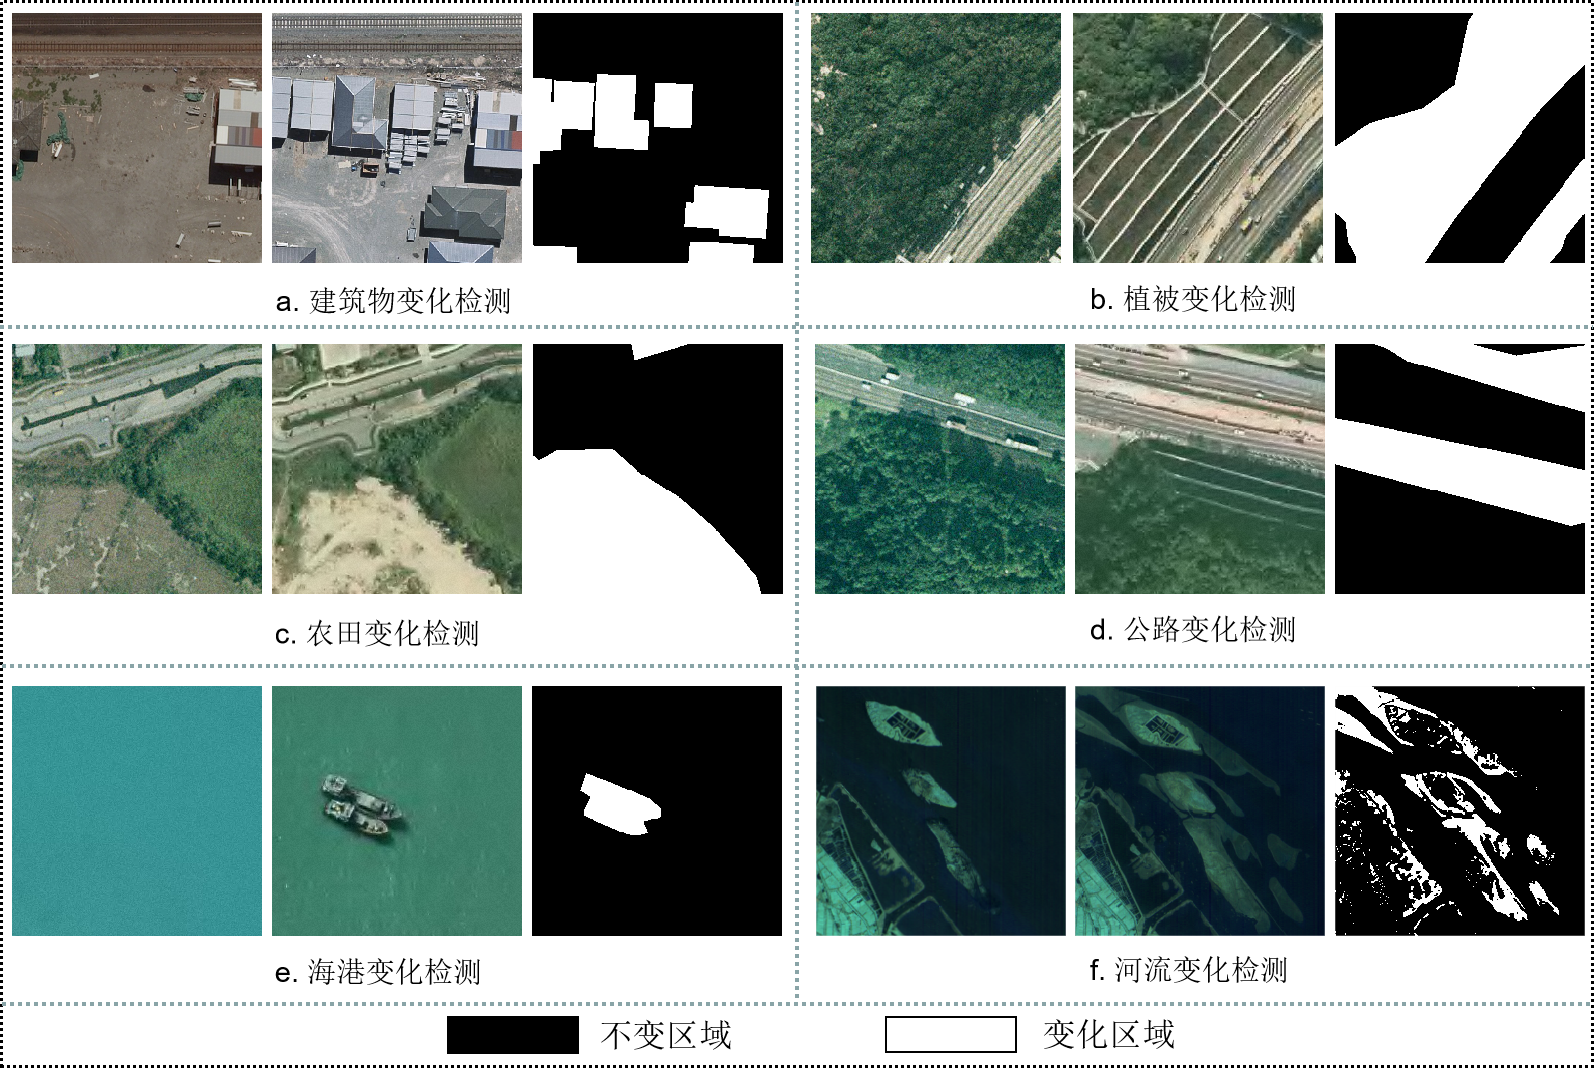
\includegraphics[scale=0.55]{images/fig1.png}
	\caption{
		变化检测在各种领域的应用。
	}
	\label{fig:background}
\end{figure}

目前,深度学习算法已经被广泛应用到各种计算机视觉任务,比如图像分类、目标检测、深度估计,以及语义分割、实例分割等与变化检测相似的密集预测任务,并且表现出了远超传统方法的优异性能。然而,基于卷积神经网络(Convolutional Neural Network, CNN)或者Transformer网络的全监督的深度学习变化检测算法都及其依赖于大量的人工标注,当有标注的训练样本减少时,模型的识别能力急剧下降。而且,变化检测任务的数据标注非常复杂,需要高精度几何图像配准和像素级精细标注,耗时耗力。这一点从目前可以获取到的公开数据集的数据规模对比就可以看出来,通常图像分类、目标检测的数据集能够达到数十万张,而变化检测的数据集规模仅在几百至几万张。为了应对这些挑战,研究人员研究了一系列方法,如自监督学习(Self-supervised learning, SSL)、无监督变化检测(Unsupervised Change Detection, USCD)、弱监督变化检测(Weakly Supervised Change Detection, WSCD)和样本生成策略(sample generation strategies)。虽然弱监督变化检测具有一定的成本效益,但它依赖于不完整或不准确的标签,这可能会引入错误信号和不可预测的噪声数据。另一方面,无监督变化检测完全不使用标注数据,而是利用数据中存在的固有联系作为监督指导,这导致它在处理分类或检测等特定任务时,由于缺乏正确的语义信息而面临挑战。样本生成策略,包括数据增强[23]、生成式对抗网络和扩散模型,经常需要模拟或合成额外的数据样本。然而,当处理有限的可用样本时,由于生成的数据多样性不足,这些方法可能会遇到约束,从而降低模型的泛化能力。半监督变化检测有效弥补了这些方法的不足,一方面它能够从有限的标注数据中学习到正确的语义信息,另一方面还能够从大量的易获得的无标注数据分布中学习到更为多样的变化特征表示,因此,半监督变化检测成为了一种更有前景的解决方案。

在此背景之下,本文着力研究了半监督变化检测算法,针对模型为无标注样本生成的伪标签可能包含错误标签从而引入额外噪声这一问题,我们从提高无标注样本的伪标签的可靠性入手进行了一系列的研究,分别从无标注样本增强、模型参数更新、伪标签生成模型、伪标签生成策略等方面进行了改进,有效地提升了伪标签的质量,从而提高了半监督变化检测算法的性能。

\section{国内外研究现状及趋势}
此前国内外学者已经在半监督变化检测算法领域进行了大量的研究,本小节将介绍与本文最相关的几个方向的研究现状,包括半监督学习,全监督遥感影像变化检测,以及半监督遥感影像变化检测的基本任务与方法和研究发展历程。
\subsection{半监督学习算法}
在实际应用场景中,无标签的数据易于获取,而有标签的数据收集起来通常很困难,标注过程也是一项极度劳动密集的工作。在这种情况下,半监督学习(Semi-Supervised Learning, SSL)是一种克服样本标注困难问题的可行方法,近年来也已经成为深度学习领域一个热门的研究方向,其旨在仅利用一小部分标记数据进行监督训练,学习到正确的语音信息,同时利用大量的无标注训练样本进行无监督训练,以提高模型的泛化性,减少过拟合现象。SSL主要包含三种策略:一致正则化(Consistent Regularization, CR)、自训练(Self Training)、生成模型以及一些包括其中多种思想的整体方法。

一致性正则化方法基于扰动一致性的概念,所谓的扰动一致性即:如果对一个未标记的数据应用实际的扰动,则预测不应发生显著变化,因为在聚类假设下,具有不同标签的数据点在低密度区域是互相分离的。这种方法首先对输入数据施加不同程度的扰动,将模型在这些输入数据上的输出之间的一致性作为训练约束。目前的三个主流的一致性正则化训练框架包括:Π-模型[35],时间集成模型[35]和平均教师(Mean-Teacher, MT)模型[32]。这几种框架都是以双分支网络作为基础架构,两个网络分支分别对扰动后的训练样本和原始训练样本进行前向推理,通过最小化两次推理的概率分布的均方误差(Mean Square Error, MSE)来优化模型参数。其中Π-模型的双分支网络之间是共享参数权重的,每次更新参数之后两个分支同步更新;时间集成模型合并时间序列上的所有输出结果,当前模型预测结果与历史预测结果的指数移动平均值(Exponential Moving Average, EMA)做均方误差计算,这有效地保留历史了信息,消除了扰动并稳定了当前值;MT模型从模型参数层面进行了平滑操作,学生模型的权重是历史模型参数的EMA集成,该模型在随后的各个领域的半监督研究中得到了应用,例如Active-Teacher用于半监督对象检测[36],[33],[37]-[39]用于半监督一般语义分割,[40]用于图像分类,[41][42]用于半监督医学图像分割。此外有研究人员也在扰动设计方面进行了探索,[43]和[25]分别在一致性正则化中应用了图像级扰动和特征级扰动。

基于自训练的半监督学习算法思想是:首先使用一个预测模型或它的某些变体来为无标注样本生成一些伪标签,将这些伪标签和有标注的数据样本混合在一起进行监督训练,提供一些额外的训练信息。一个最为关键的问题就在于伪标签的可靠性,因为这直接影响了模型的训练效果,因此大量的研究从此处入手,研究了生成高质量伪标签的方法。[44]采用一个设定的概率阈值作为选择标准,预测概率小于此阈值的类别标签直接被丢弃。ST++[45]开发了一种多层自训练结构,每个阶段选择一批高质量的伪标签参与到训练,反复进行此挑选和训练过程,直到所有未标记的样本都得到了利用。[46]计算出伪标签中每个像素的信息熵,使用一个恒定的熵值作为过滤阈值,排除那些不可靠的伪标签。此外还有一种协同训练(Co-training)框架\cite{co-training},这种框架包含两个模型,分别为彼此提供伪标签。

基于生成模型的方法旨在利用生成模型对数据的分布进行建模,从而推断出未标注数据的潜在信息。半监督变分自编码器\cite{semiVAE}是变分自编码器(Variational Autoencoder, VAE)在半监督学习中的一种扩展方法,添加了一个分类器来学习语义信息,首先VAE从标注样本集中学习一个真实的数据分布,然后在大量的无标注样本上基于分类器分类结果去指导模型学习一个更为丰富的潜在分布。Ren等人[]利用生成对抗策略训练了一个能够生成共配准图像的生成器,从原始图像高维特征空间中采样,从特征空间分布的上界和下界之间按照策略选择一些特征向量生成高质量配准图像,从而后续只需用通过特征融合方法即可找出变化区域,并且扩充了学习到的特征空间。Bandara等人在大规模数据集上预训练了一个Denoising
Diffusion Probabilistic Models(DDPM),利用其具有强大表征能力的编码器进行双时图像的特征提取以提高变化检测性能。

通常情况下,实际应用中更多采用的是整体方法(Holistic Methods),即在一个框架中整合前述的 SSL 的主要方法,从而获得更好的性能。比如[33]、[38]-[40]和[45]这些研究工作。其中最为经典的是FixMatch\cite{sohn2020fixmatch},提出了一种基于伪标签和一致性正则化的简单而有效的整体方法。进一步,Yang等人根据分类和分割任务的差异,增加了一种新的前馈流即特征摄动,以及一种极强的增强摄动流,通过多一致性约束构造更广阔的扰动空间。此外,他们同期关于半监督语义分割的另外两项研究考虑了在半监督语义分割训练中加入自适应调整机制,但他们的视野局限于训练数据,遗憾的是他们没有考虑更高层次的模型训练。

\subsection{基于深度学习的遥感影像变化检测}
受深度学习在各领域取得的巨大成功所启发,近十年在变化检测领域也涌现出了许多经典的工作,推动了遥感影像变化检测研究的发展,下面本小节将按照大致的时间顺序分别介绍基于CNN的变化检测方法、基于Transformer的变化检测方法以及近期出现的基于大模型的变化检测方法。
\subsubsection{基于CNN的变化检测方法}
CNN引入了卷积和池化网络层,使其能够有效地捕获数据中的空间特征和局部关系,同时通过深度网络结构层层提取更抽象的高维特征,经典的CNN架构包括LeNet-5、AlexNet、VGG、ResNet等。研究人员利用双分支孪生网络分别对两幅时相图像进行处理,提取高维特征,然后进行特征融合,识别出双时相图像对之间的差异。最为经典的工作是Daudt 等人\cite{daudt2018FC-EF}在2018年使用全卷积网络构建了基于UNet的架构及其两个孪生变体,这三种变化检测框架分别是FC-EF、FC-Siam-conc、FC-Siam-diff,每种框架都采用了不同的特征融合策略,其中FC-EF是在输入层面首先对双时相图像进行了图像级别的融合,另外两种都是对从双时相图像对中抽取的高维特征进行融合。Shi等人\cite{shi2021DSAMNet}提出的DSAMNet在每个多尺度特征融合阶段添加了卷积块注意模块(Convolutional Block Attention Modules,CBAM),这种轻量级的注意力机制从空间和通道两个维度上对特征之间的关系进行了建模,动态地调整了特征图地权重。Zhang等人\cite{zhang2023MFNet}提出了一个互特征学习网络——MFNet(Mutual Feature-Aware Networks),提出的对称变化特征融合模块弥补了此前差分特征融合造成的信息丢失问题,同时通过在编码阶段提前引入差异感知,使得编码器更加聚焦于对潜在变化区域的特征学习。Fang等人\cite{fang2021SNUNet}将孪生网络和稠密连接的NestedUNet网络结合到了一起,浅层特征和深层特征之间紧凑的信息传输减少了特征抽取中的位置信息丢失。Zheng等人提出的ChangeStar\cite{zheng2021changestar}通过构造伪配准图像对,以语义分割方式来处理两幅图像,以单时相图像来训练双时相图像对变化检测模型,减少了对特征融合和图像配准的依赖。总的来说,基于CNN的监督变化检测方法大多侧重于特征融合模块的设计或者精巧的编码器设计,以更加精确地表示变化特征。
\subsubsection{基于Transformer的变化检测方法}
Transformer 是一种基于自注意力机制的深度学习模型,最初由 Vaswani 等人在 2017 年提出\cite{vaswani2017transformer},首次用于自然语言处理任务中的序列到序列(Seq2Seq)建模,尤其是在机器翻译任务中取得了革命性突破。其核心特性是完全抛弃了传统的循环神经网络(RNN)和卷积神经网络(CNN),以自注意力机制和全连接网络为基础,显著提高了模型在长程依赖任务中的效率和性能。随着Google Research 于 2020 年提出了Vision Transformer (ViT)\cite{dosovitskiy2020vit},首次将Transformer网络应用到了计算机视觉领域,其迅速成为了计算机视觉领域的新宠方向,在变化检测领域亦是如此。Chen等人首先将VIT引入了变化检测任务,提出的BIT\cite{chen2021BIT} 是一种基于原生 Transformer 架构的网络,旨在通过Transformer对双时相图像的时空上下文进行建模。然而,该模型直接采用原生 Transformer 的解码器,未充分利用浅层特征,这限制了其性能。相比之下,Li 等人提出的TransUnet\cite{li2022transunetcd}引入了 UNet 风格的解码器,取代了 Transformer 原有的解码方式,通过融合上一阶段的特征图逐步恢复至原始尺寸,从而显著提升了模型的表现。NVIDIA 提出的 SegFormer \cite{xie2021segformer}是一种基于 Transformer 的通用语义分割架构,利用轻量级编码器实现多尺度特征提取。受其启发,Bandara 等人设计了 ChangeFormer\cite{bandara2022transformer},该模型引入了针对变化检测任务的特定模块,通过卷积操作学习双时相特征图之间的变化关系。相比传统方法,ChangeFormer展现了更高的精度和鲁棒性。Jiang等人提出的VcT\cite{jiang2023vct}将每个像素作为一个图节点,利用图神经(GNN)网络对所有节点组成的结构化信息进行建模,挖掘具有共同背景信息的可靠token,而不是像以往手动设置固定token,更具针对性的特征学习提高了检测的效率和准确性。

一些研究发现,在变化检测中,由于数据有限,纯Transformer模型可能无法发挥其全部潜力。因此还有一些研究将CNN和Transformer结合在了一起,使得两种模型的优点能够互补,既可以利用CNN强大的局部信息捕捉能力,又能够利用Transformer兼顾对全局关系的建模,实现全局特征和局部特征学习的统一。比较经典的工作有Jiang提出的MSFCTNet\cite{jiang2024cnntranscd}和Li等提出的MCTNet\cite{lwm2023cnntransCD2}和ConvTransNet\cite{lwm2023cnntransCD}。这类方法总体思想基本一致,但这些研究人员分别从不同方向对CNN与Transformer的高效信息交互进行了改进和创新。
\subsubsection{基于大模型的变化检测方法}
近年来,大模型(Large Models)的发展成为人工智能领域的核心热点之一。这些模型以大规模参数、海量数据和复杂架构为特征,在自然语言处理、计算机视觉、强化学习等领域展现出卓越性能。它们通常基于自注意力机制(Self-Attention)驱动的Transformer模型,通过在大规模数据集上边的自监督预训练,获得了强大的通用表征提取能力,虽然这些模型和上一小节同属Transformer类型,但由于其带来的变革性突破,本小节将单独分析基于大模型的变化检测研究。自从自然语言处理领域的BERT、GPT问世并引起广泛关注以后,计算机视觉领域的预训练大模型也迅速地出现在了人们的眼前。其中SAM\cite{kirillov2023SAM}(Segment Anything Model)是图像分割通用大模型的开篇之作,以其强大的零样本推理能力和无需微调的交互式分割,被认为彻底颠覆了传统的深度学习方法。Li等人\cite{li2024LM}最早提出了结合大模型进行变化检测的新范式,提出了一个包含冻结基础模型(如CLIP\cite{radford2021clip}、SAM等)、双时态适配分支(Bi-TAB)以及它们之间的桥接模块三部分的双时态适配网络(BAN),将大模型的大量先验知识注入到了变化检测模型。Ding等人\cite{ding2024SAMCD}通过训练一个轻量级的适配器网络(Adapter)来更具针对性地利用SAM在遥感影像场景中强大的视觉表示能力对双时相图像进行特征提取。Liu等人\cite{liu2024changeagent}将大语言模型和变化检测模型结合起来,提出了一个变化检测智能体(Change-Agent),能够输入文本和图像两种模态的数据,按照输入指令交互式地检测感兴趣的变化区域。Dong等人\cite{dong2024changeclip}同样基于Clip进行了多模态变化检测的研究,他们将图像-文本编码的结果与解码阶段的视觉特征相结合,从而增强了图像的语义。Zheng等人\cite{zheng2024SAC}利用SAM强大的零样本扩展能力,基于构建的点提示以及SAM提取的特征空间在图像内和图像间的潜在相似性,进行无需训练的零样本推理,首次提出并应用到了零样本变化检测任务。但是这和传统意义上的零样本任务任然有差别,就是需要人工对每幅图像进行点提示的标注。
\subsection{半监督遥感影像变化检测}
对大量图像进行变化检测的精细标注非常耗时,目前解决此问题的方法主要集中在半监督变化检测上(Semi-supervised Change Detection,SSCD)。与第1.2.1小节的半监督算法研究类似,SSCD也主要分为两大类别,其一是基于一致性正则化的方法,其二是基于生成对抗模型(Generative Adversarial Network,GAN)的方法。

在一致性正则化方面,在变化检测中引入平均教师模型最早是由Bousias等人提出的[47]。然而,最初的实验结果并没有显示出相当大的潜力,因为与仅使用有限数量的标记数据进行完全监督学习的基准相比,这种SSCD方法存在不足。甚至随着真实标注数据越来越多,这种与全监督训练之间的性能差距仍在继续扩大。以此为基础,Mao等人[48]分别对教师模型和学生模型的输入进行了强、弱增强操作。此外,他们制定了一个额外的教师虚拟对抗训练组件,以进一步减少伪标签噪音的负面影响。此外,有的其他半监督方法使用单模型或具有共享权重的双分支模型。如Sun等[49]引入了孪生网络。他们结合了基于伪标签的额外自训练,采用阈值过滤来消除低质量的伪标签。这种过滤背后的基本原理在于低置信度的伪标签引入的潜在噪声,这可能对自训练产生不利影响。Hafner等人提出了一种双任务SSCD框架,该框架结合了建筑物分割和变化检测这两个密切相关的下游任务。他们在Siamese分割网络和变化检测网络产生的两个变化检测掩码之间设计了一种新的一致性约束。Bandara等[25]探索了新的正则化项,即基于特征的扰动,在特征层面应用各种数据扰动来扩展一致性约束的分布空间。该方法充分利用了未标记样本中嵌入的信息,在最近的工作中,Zhang等人[27]对未标记数据集施加了类一致性和特征一致性两个约束。通过将未标记样本在变化类和不变类上的特征表示对齐,模型可以从更接近真实分布的特征空间中学习,这使得他们极大地改进了SSCD的性能。

其他方法主要利用GAN这种生成模型,它最初是由Goodfellow在2014年提出的[51]。一些方法使用GAN来学习接近真实标记数据的特征分布空间[26],[52]- [54];另一部分使用GAN生成数据样本[55],[56];在最近的工作中,比较值得注意的研究是[18]提出了一种新的变化检测范式,将无监督、弱监督、区域监督和完全监督的变化检测统一到了一个端到端的框架中,在无监督变化检测中,主要目标被定义为最小化一个区域,使得生成网络可以在屏蔽该区域后产生与另一个时间的图像相似的图像。对于弱监督和新提出的区域监督变化检测任务,关键思想在于最小化一个区域,使判别网络在屏蔽该区域后无法区分真实不变图像对。虽然这些努力在SSCD中取得了巨大的成功,但GAN的高度不稳定训练使得超参数调整变得具有挑战性。此外,梯度消失的问题经常出现在训练阶段,以及如果没有实施额外的训练技术,鉴别器的强判别能力可能导致GAN的生成器和鉴别器之间的性能不平衡。因此,实现理想的最优场景是具有挑战性的,这使得该方法的基本应用有些复杂。

\section{本文主要内容及结构安排}
本文着力研究半监督变化检测任务,在少量有标注训练数据上学习正确的语义信息并在大量且易获得的无标注训练样本上学习到一个更加丰富的特征空间分布。其中一个关键问题就在于能否减少无标注样本训练中不可避免的噪声问题,这有两种解决方案:通过改善伪标签的质量来提高半监督变化检测的性能;从特征层面构造正则化项从而排除错误伪标签的重要影响。本文从这两点入手,主要研究内容如下:

1)基于伪标签评估的自适应半监督变化检测。针对大量的无标注样本中不同样本个体之间存在很大的差异,模型为这些具有不同难易程度的样本生成的伪标签可靠性也不尽相同。本算法设计了一种自适应动态学习策略AdaSemiCD,旨在提高伪标签的准确性并简化训练过程。我们的框架结合了传统的半监督训练方法,并辅以两个创新的功能模块AdaFusion和AdaEMA。首先,我们利用AdaFusion在单个样本水平上对不确定性高的样本区域进行改造,从而提高伪标签的准确性。其次在AdaEMA模块中引入了模型级参数更新的自适应选择过程,使模型能够充分集成优越的参数。大量的实验结果表明了我们所提出的方法能够极大地改善伪标签的质量,使得变化检测性能更好。

2)基于大模型先验的半监督变化检测。针对变化检测网络为无标注数据生成的伪标签质量不足可能引入大量额外噪声的问题,我们通过构建一个在包含遥感数据的大规模数据集上进行过预训练的大模型辅助模块,引入大量的先验知识;同时利用通用分割大模型在目标边界上的强大分割能力,通过几种不同的融合策略,从单时相分割掩码生成双时相变化检测掩码,以改善伪标签质量。实验表明从预训练通用分割大模型引入先验知识能够达到更好的变化检测性能。

3)基于特征对齐的半监督变化检测。

本文的章节结构安排如下:

第一章首先系统性地阐述了变化检测任务的应用场景和研究价值,以及半监督变化检测算法的研究背景和意义,然后梳理了目前国内外关于半监督学习、深度变化检测、半监督变化检测的研究进展和主流方法,最后介绍了本文的主要研究内容和文章结构安排。

第二章首先介绍了本文研究工作中用到的一些骨干特征提取网络和预训练大模型,之后对本研究工作中进行对比的几种经典半监督变化检测算法进行了阐述,最后详细介绍了本研究中采用的实验指标和用到的数据集。

第三章基于伪标签评估的自适应半监督变化检测工作介绍。首先介绍了模型的整体框架以及训练流程,随后详细介绍了设计的伪标签评估指标,以及基于此指标设计的两个自适应模块。最后在实验部分报告了该研究方法在十个公开数据集上取得的实验结果,并与其他经典半监督变化检测算法在定性和定量上进行了公平的对比,最后通过消融实验证明了每个模块的有效性。

第四章基于大模型先验的半监督变化检测工作介绍。首先介绍了模型整体框架和设计的三种变化掩码生成策略,之后介绍了实验设置以及展示了取得的实验指标结果和可视化结果,通过大量的对比实验结果验证了本工作的有效性。

第五章基于特征对齐的半监督变化检测工作介绍。首先介绍了模型整体框架,以及我们对图像间的同类特征潜在相似性的探究,并随后介绍了以此为基础结合预训练大模型提出的多源特征对齐方法,最后通过大量的对比实验,验证了本章所提方法的优越性。

第六章总结与展望。从全局角度总结了本文的主要研究工作,并对未来半监督变化检测领域可以继续改进创新之处做出了展望。
\cleardoublepage
\chapter{相关技术}

本章将介绍本文基于深度学习的半监督变化检测算法研究中所用到的相关技术,为后续章节做好铺垫。具体包括:2.1小节中详细介绍本文几个研究工作中用到的深度神经网络,包括卷积神经网络,Vision Transformer以及Segment Anything Model的网络结构等;2.2小节对上一章节研究现状中概括性介绍的几个经典半监督变化检测算法进行了详细的阐述;2.3小节对本文所有实验所采用的实验指标进行了解释;2.4小节对本文所有进行实验的公开数据集进行了详细介绍。

\section{深度神经网络}
深度神经网络(Deep Neural Network, DNN)是一种以多层神经元结构为基础的机器学习模型,广泛应用于诸多领域,包括计算机视觉、自然语言处理、语音识别以及推荐系统等。基于任务需求,DNN衍生出多种具体架构,例如用于图像处理的卷积神经网络(Convolutional Neural Network, CNN),在序列建模中表现优异的循环神经网络(Recurrent Neural Network, RNN),以及基于多头自注意力机制对全局关系进行建模的Transformer架构。虽然神经网络并不是本文的主要研究方向,但是由于后续研究中会多次涉及卷积神经网络中比较经典的网络模型,因此在本小节将介绍后续研究工作所用到的几种骨干特征提取网络,即ResNet,Vision Transformer,以及基于Transformer预训练的通用分割大模型Segment Anything Model的模型结构。
\subsection{ResNet}
在深度学习的发展过程中,研究者们发现随着卷积神经网络层数的增加,模型的表达能力理论上会不断增强。然而,在实际训练深层网络时,却遇到了两个主要问题:(1)梯度消失和梯度爆炸问题;(2)退化问题。这些问题阻碍了深层神经网络的发展,最终何等人\cite{He2015ResNet}提出了残差网络(Residual Network, ResNet),通过在网络层之间引入残差连接使得前层的输出直接加到后层的输出上,如公式\ref{eq:resnet}所示,其中$x$代表输入特征,下标表示网络层序号,$W_l$代表第$l$层的参数,$F\left(x_l,W_l\right)$表示卷积映射。通过这种方式,梯度在反向传播时可以通过跳跃路径直接传播到前层,避免了梯度逐层递减的问题,从而缓解了梯度消失,同时即使一些层对学习贡献较小,残差连接可以保证网络的性能至少不会发生退化现象。
\begin{equation}
  \label{eq:resnet}
  x_{l+1} = x_l + F\left(x_l,W_l\right)
\end{equation}

此外残差结构还减少了优化深层网络的难度,是网络结构更加复杂、网络层数进一步增加成为了可能,从而显著提升了卷积神经网络的表征能力和性能,推动了深度学习向更深、更强的方向发展。比如何等人同时提出了具有不同网络层数的ResNet,包括ResNet-18、ResNet-34、ResNet-50、ResNet-101以及ResNet-152,它们的网络架构如图\ref{fig:resnet}所示。
\begin{figure}[htb]
  \centering
  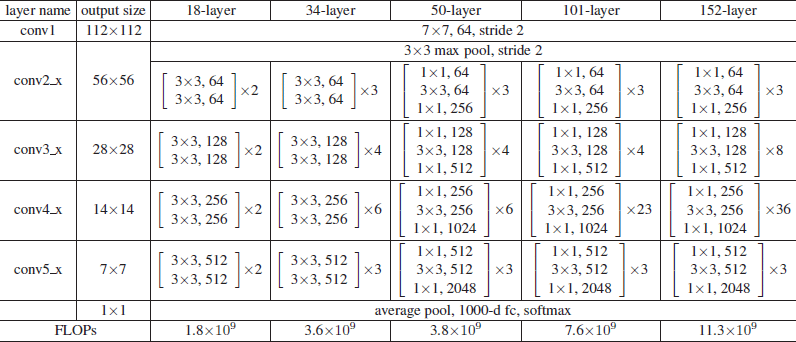
\includegraphics[scale=0.55]{images/resnet.png}
  \caption{
    不同深度的ResNet网络层次架构\cite{He2015ResNet}。
  }
  \label{fig:resnet}
\end{figure}
此外后续还有研究提出了一些ResNet变体,例如ResNetV2\cite{2019resnetV2}和ResNeXt\cite{xie2017ResNeXt}。根据网络深度和任务需求,ResNet中存在两种经典的残差块,一种是用于浅层网络(如ResNet-18和ResNet-34)的基本残差块(Basic Residual Block),包含两个$ 3\times3 $的卷积层和直接的跳跃连接,一种是用于深层网络(如ResNet-50、ResNet-101和ResNet-152)的瓶颈残差块(Bottleneck Residual Block),它将两个 $ 3\times3 $ 的卷积层替换为$1 \times 1$,$3 \times 3$,$1 \times 1$ 的卷积网络,其中前后两个$1 \times 1$卷积层分别用于降低和恢复特征通道数,有效地减少了计算量和参数量,网络结构如图\ref{fig:resblock}所示。本文研究工作中采用的是ResNet-50,一共包含4个卷积阶段,每一个阶段中分别有3,4,6,3个瓶颈残差块。


\begin{figure}[htb]
  \centering
  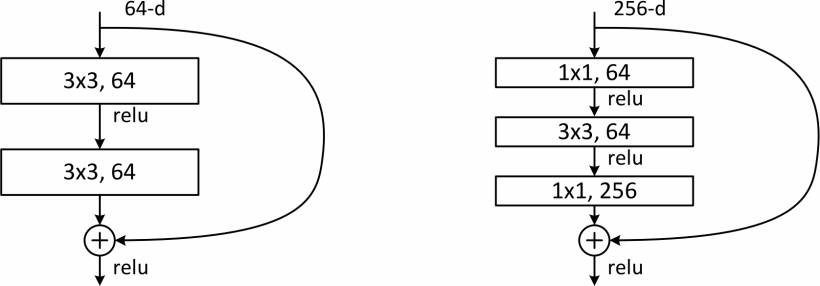
\includegraphics[scale=0.55]{images/res-block.png}
  \caption{
    两种残差块的网络结构\cite{He2015ResNet}。
  }
  \label{fig:resblock}
\end{figure}

\subsection{Vision Transformer}
虽然CNN在计算机视觉任务(如图像分类、目标检测、语义分割等)中占据主导地位,然而其在捕捉长距离依赖和全局信息时存在很大局限性。与此同时,Transformer在自然语言处理(Natural Language Processing, NLP)领域取得了显著成功,尤其是在任务如机器翻译和文本生成中。Transformer的核心优势是通过自注意力机制(Self-Attention Mechanism)捕捉输入数据中全局依赖关系。受此启发,Dosovitskiy等人\cite{dosovitskiy2020vit}对Transformer进行改进使其能够适配计算机视觉任务,形成了Vision Transformer(ViT)架构。这种方法首次完全摆脱了卷积操作,在多个基准测试中展现出与甚至超越CNN的性能。它的核心思想是将图像分割为固定大小的图像块(patches),并将每个块视为一个独立的“词”,类似于NLP中的词嵌入,这些图像块嵌入向量通过Transformer的自注意力机制进行处理,从而实现对图像的全局理解。
\begin{figure}[htb]
  \centering
  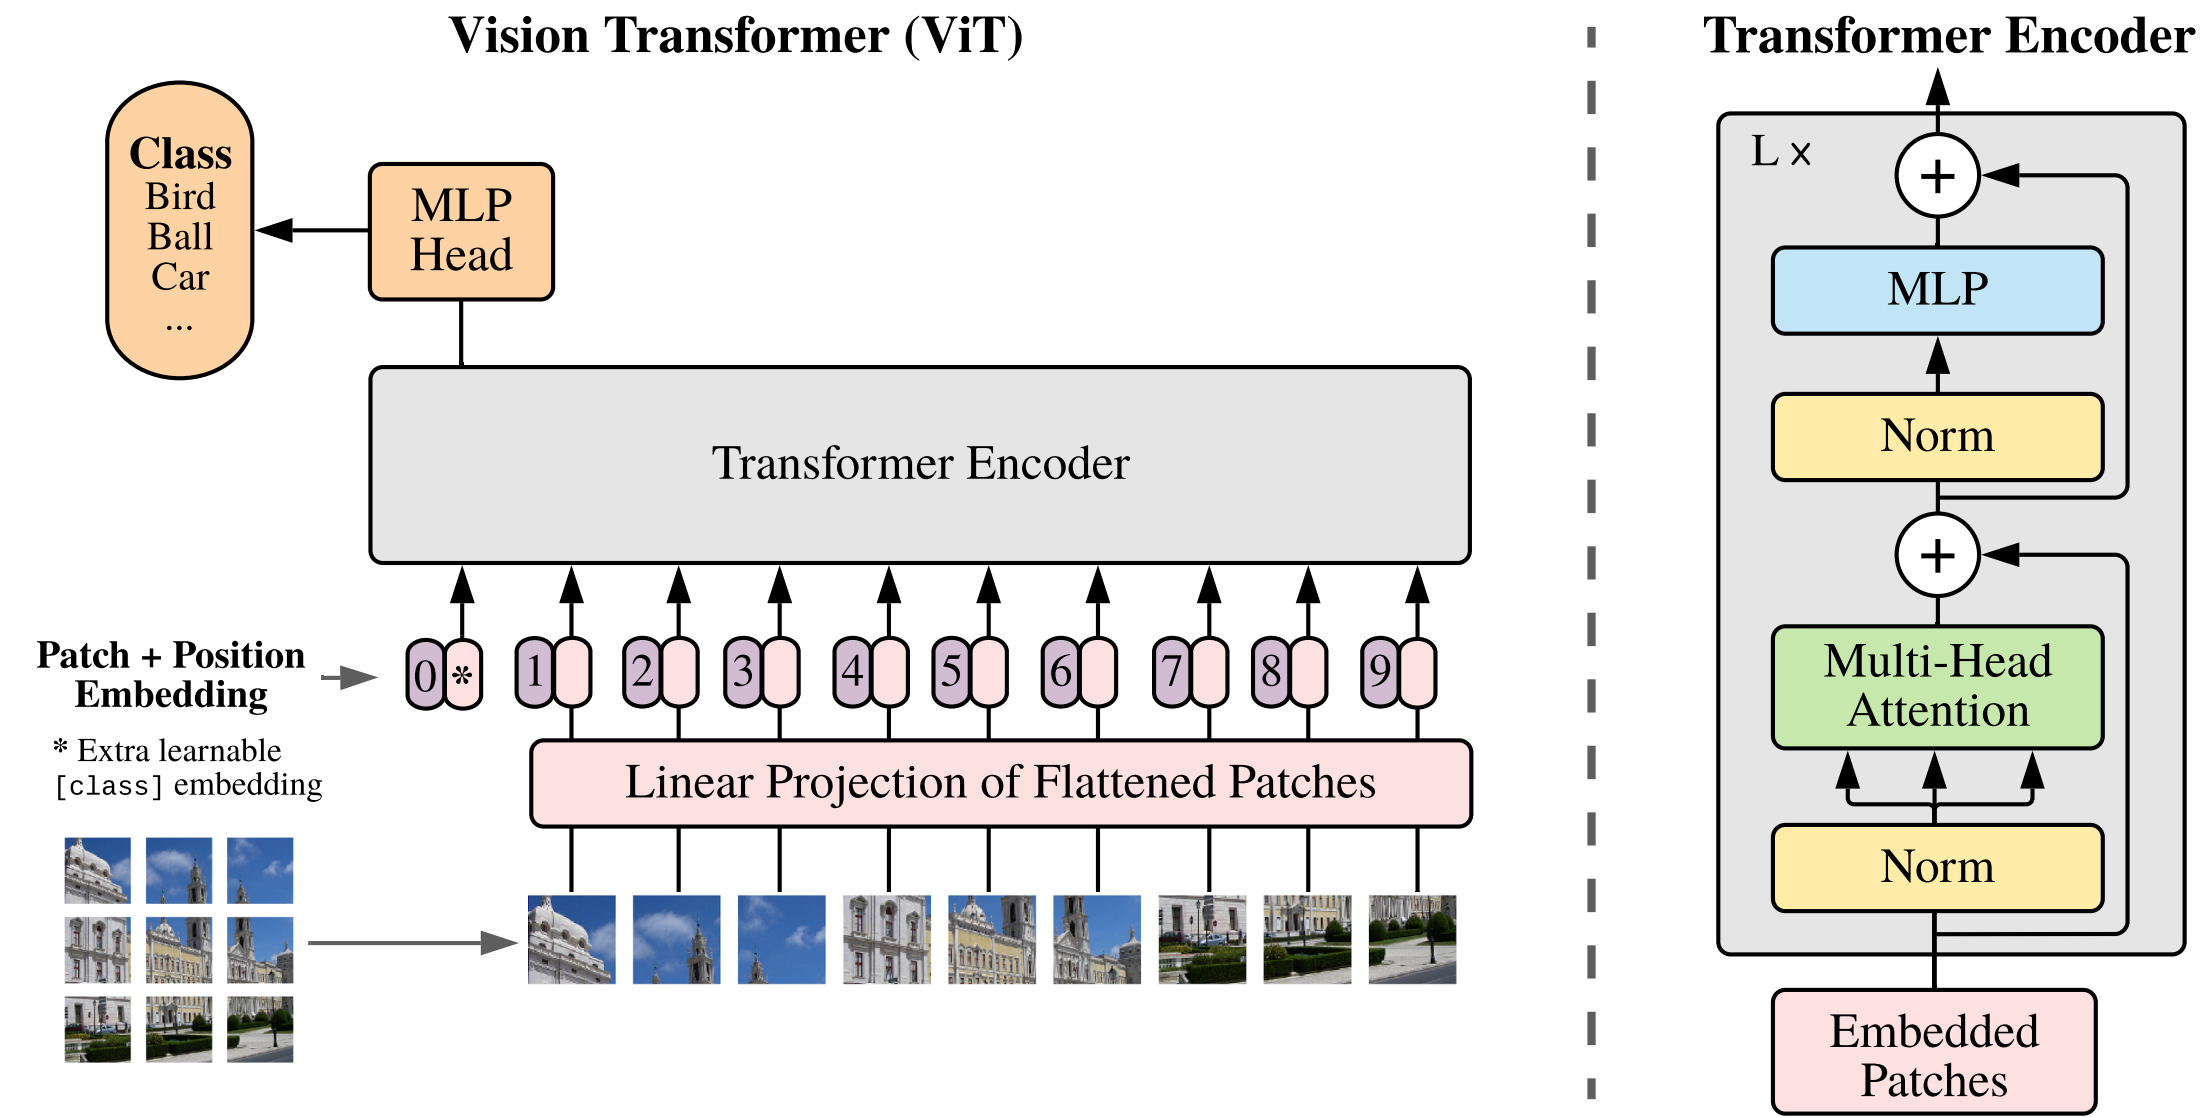
\includegraphics[scale=0.55]{images/ViT.png}
  \caption{
    Vision Transformer网络框架\cite{dosovitskiy2020vit}。
  }
  \label{fig:ViT}
\end{figure}

ViT的网络结构如图\ref{fig:ViT}所示,输入的图像首先被分割为大小为$P\times P$的非重叠图像块(patches),每个块展平为一维向量并通过线性映射嵌入到D维特征空间,假设图像大小为$H \times W$且通道数为$C$,则切割后共生成$N=\frac{H}{P} \times \frac{W}{P}$个图像块,这些块被视为Transformer的输入“词”。为保留块之间的空间顺序信息,ViT为每个嵌入向量添加一个可学习的位置编码,此外,在输入序列的起始位置插入一个特殊的分类标识符([CLS] Token),该标识符的嵌入向量用于最终的分类输出,如公式\ref{eq:embeding}。经过嵌入和位置编码后的输入序列被送入由L层组成的Transformer编码器,每层包含多头自注意力机制(Multi-Head Self-Attention, MHSA)和前馈网络(Feed-Forward Network, FFN)。在MHSA中,每个图像块嵌入向量通过查询(Query)、键(Key)和值(Value)矩阵生成注意力权重,用以捕捉图像块间的全局关系,表示为公式\ref{eq:attention}。其中$Q$、$K$、$V$是从输入嵌入计算得到的查询、键和值矩阵,$\sqrt{d_{k}}$是注意力头的维度。每个Transformer层都配有残差连接和层归一化,用以提高训练稳定性。经过L层编码器后,分类标识符的嵌入向量$z_{0}^{[C L S]}$被用作图像的全局表示,并通过一个全连接层映射到类别数的维度,最终通过Softmax函数生成分类概率,如\autoref{eq:softmax},其中$W_{\text {head }}$和$b_{\text {head }}$为分类头的参数。
\begin{equation}
  \label{eq:embeding}
  z_{0}=\left[z_{0}^{[C L S]} ; z_{0}^{1} ; z_{0}^{2} ; \ldots ; z_{0}^{N}\right]+E_{\mathrm{pos}}
\end{equation}
\begin{equation}
  \label{eq:attention}
\operatorname{Attention}(Q, K, V)=\operatorname{softmax}\left(\frac{Q K^{\top}}{\sqrt{d_{k}}}\right) V
\end{equation}
\begin{equation}
  \label{eq:softmax}
  \hat{y}=\operatorname{Softmax}\left(z_{L}^{[C L S]} W_{\text {head }}+b_{\text {head }}\right)
\end{equation}

ViT摒弃了传统卷积操作,采用自注意力机制实现图像全局特征的高效建模,其模块化和可扩展的架构使其在大规模数据集和高效计算资源支持下展现出优异性能。然而,ViT在小规模数据场景中仍面临一定挑战,主要体现在模型对训练数据的需求较高和计算效率的限制。因此,针对训练数据稀缺的情况,结合半监督学习算法是一种具有潜力的研究方向,通过充分利用未标注数据,有望显著提升ViT在小数据集场景下的表现。
\subsection{Segment Anything Model}
自然语言处理领域中基于Transformer的大模型(如GPT和BERT等)展现了跨任务和跨领域的通用性,这进一步推动了视觉领域对通用大模型的需求。受此启发,Meta AI提出了Segment Anything Model\cite{kirillov2023SAM}(SAM),旨在实现对任意图像或视频中的对象进行高效、精准的分割,而无需对具体类别或场景进行额外的训练。其设计理念与通用大模型相似,即通过大规模数据集预训练,使模型具有广泛的泛化能力,能够零样本或少样本适应新任务。其核心思想是通过一个提示驱动(prompt-driven)框架,允许用户通过灵活的提示方式(如点、框、文本描述等)来指定感兴趣的区域,从而实现高度交互性和可控性。SAM的提出不仅是计算机视觉技术发展的延续,更标志着分割任务从任务特定模型向通用模型转变的关键一步,开启了视觉任务中的“分割一切”。
\begin{figure}[htb]
  \centering
  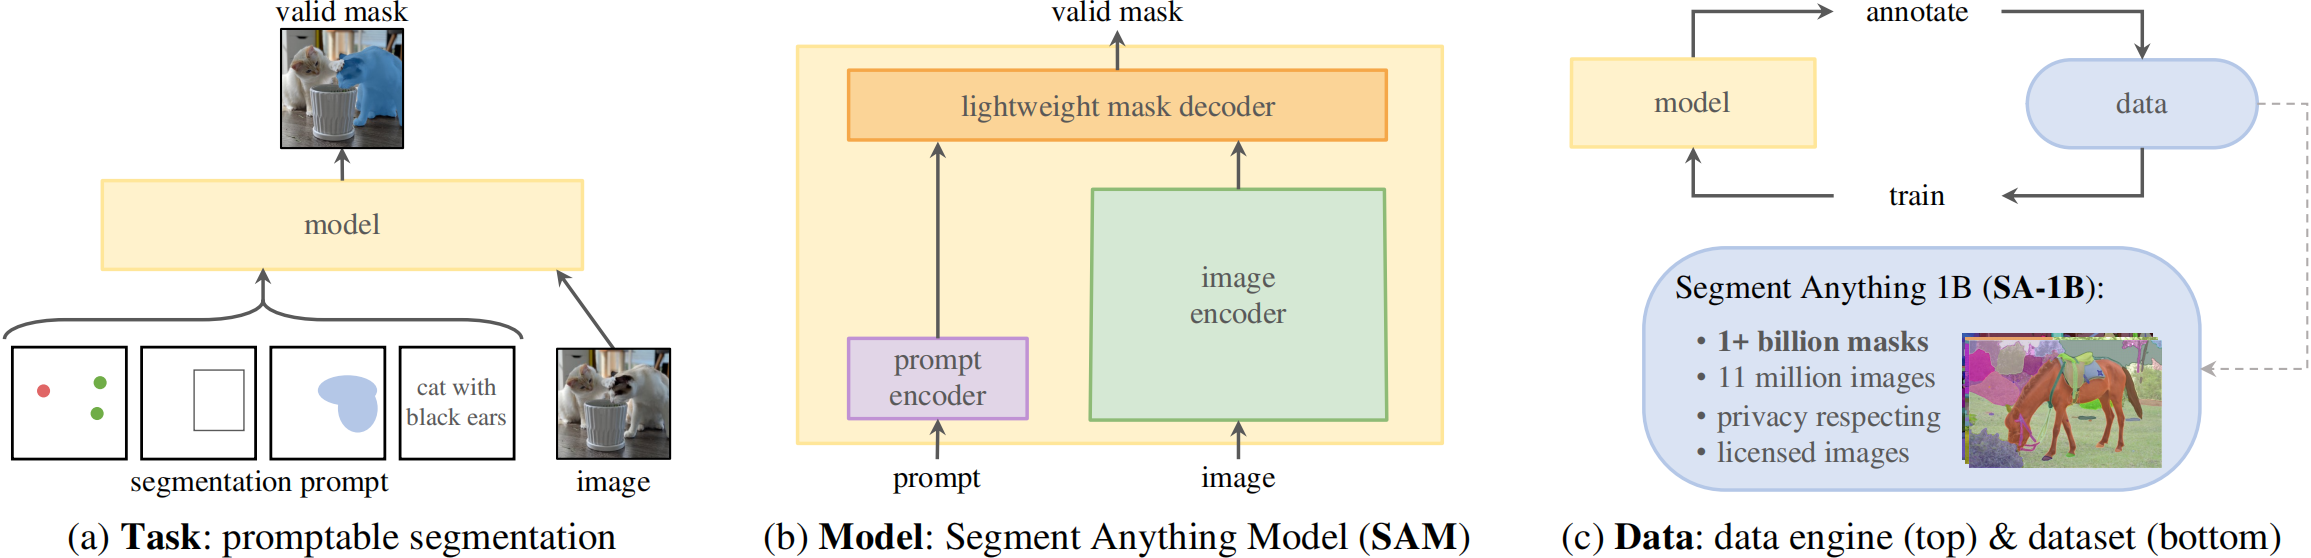
\includegraphics[scale=0.55]{images/SAM1.png}
  \caption{
    分割一切基础模型架构\cite{kirillov2023SAM}。
  }
  \label{fig:SAMfram}
\end{figure}

为了实现这一目标,SAM引入了三个相互关联的组件来构建了分割的基础模型:一个基于提示的分割任务、一个通过数据标注提供动力并能够通过提示工程实现一系列任务零样本迁移的分割模型(SAM),以及一个用于收集数据集SA-1B的数据引擎,如图\ref{fig:SAMfram}。
SAM的显著特性是支持多种类型的用户输入作为提示,包括:(1)单点提示,通过在目标对象上指定一个点,SAM能够快速分割该点所属的对象;(2)多点提示,当用户提供多个点时,模型能够根据点之间的关系生成更精确的分割;(3)框提示,通过提供一个边界框,模型可以分割框内的目标对象;(4)文本提示,与自然语言描述结合,通过文本指定需要分割的对象类别。这种灵活的提示驱动机制使SAM在复杂场景下能够通过用户少量交互即可实现高效分割。SAM的网络架构主要由三个主要部分组成,分别是图像编码器(Image Encoder),提示编码器(Prompt Encoder)以及掩码解码器(Mask Decoder)。其中图像编码器就是基于前文介绍的强大的ViT模型,用于提取高质量的全局图像特征,图像编码器在输入时对整幅图像进行一次性编码,生成具有全局上下文的多尺度特征嵌入。提示编码器用于编码用户提供的提示信息,包括点、框或文本等。点或框提示会被转换为位置嵌入,而文本提示则通过专门的文本编码器进行嵌入,提示编码器的设计使模型能够灵活适应多种提示形式。掩码解码器负责将图像编码器生成的全局特征与提示编码器的提示信息融合,生成与提示相关的分割掩码,如图\ref{fig:SAMfram}中所示的过程。此外SAM的强大性能得益于在一个规模空前的大型分割数据集上进行的预训练。该数据集包含超过11亿个图像-分割掩码对,覆盖了广泛的对象类别、场景和视觉条件。通过大规模预训练,SAM获得了卓越的通用性和泛化能力,能够分割未见过的对象或复杂场景中的目标,而无需进一步微调或额外标注。
\begin{figure}[htb]
  \centering
  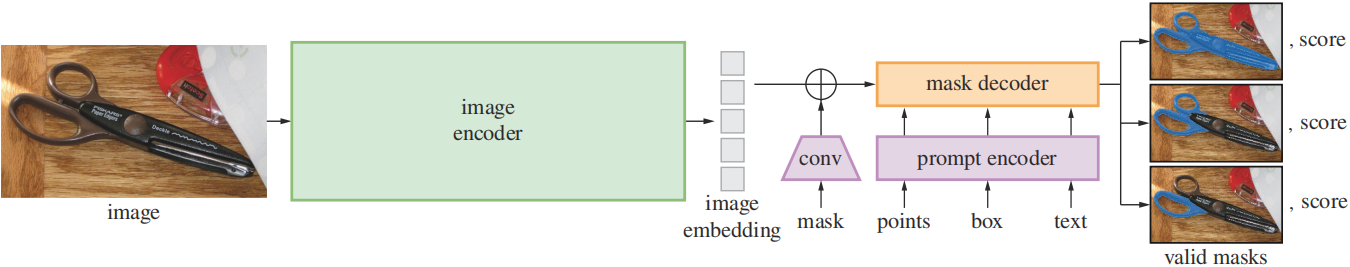
\includegraphics[scale=0.9]{images/SAM.png}
  \caption{
    Vision Transformer网络框架\cite{kirillov2023SAM}。
  }
  \label{fig:ViTfram}
\end{figure}

SAM是一项具有里程碑意义的技术,它通过灵活的提示驱动机制和大规模预训练,构建了一个适用于广泛视觉场景的分割模型。其强大的零样本推理能力和边界预测能力使得其可以不用微调直接用于其他场景和任务,并提供先验知识和辅助推理来优化性能,因此本文的研究工作中引入了SAM模型。
\section{经典半监督变化检测算法}
\subsection{RCR}
RCR(Revisiting Consistency Regularization)由Bandara等人\cite{bandara2022RCR}提出的,它们基于聚类假设构建了一个更加广阔的特征扰动空间,这种特征扰动一致性正则化使得模型具有更加强大的泛化能力。本文的研究工作的代码是基于RCR的变化检测网络和训练框架以及前文提到的平均教师模型改进实现的,因而有必要在本小节详细介绍RCR方法。

(1)网络框架。

总体框架如图\ref{fig:RCRfram}所示,主要包括三个模块:
1)编码器,用于提取前时相图像和后时相图像的隐藏特征表示。
2)特征差分模块,用于获取变化前和变化后图像的隐藏特征表示Fd的差异。
3)解码器,从隐藏的差异特征表示预测变化掩膜。
\begin{figure}[htb]
  \centering
  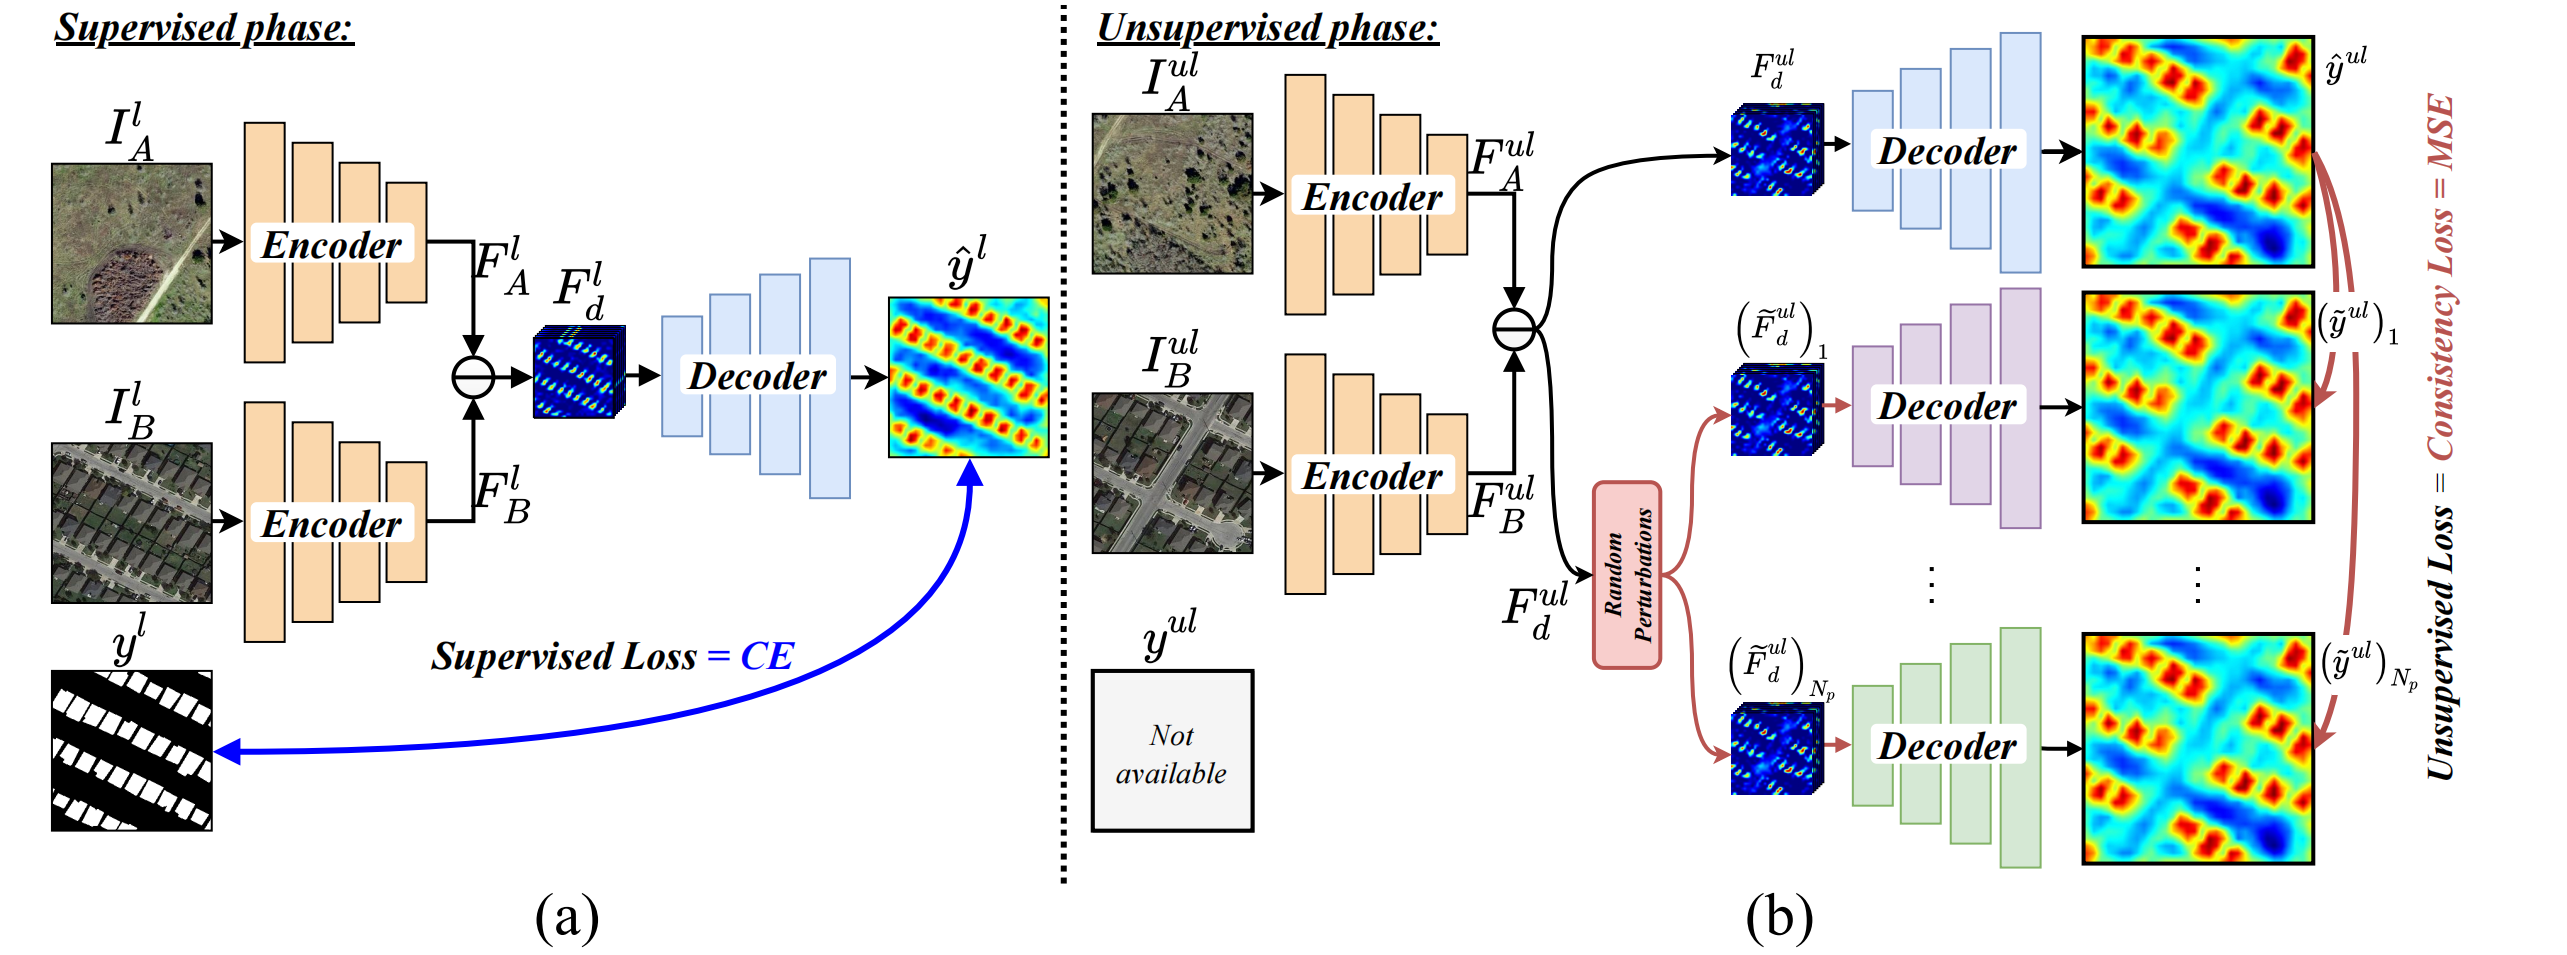
\includegraphics[scale=0.5]{images/RCRframe.png}
  \caption{
    RCR网络框架\cite{bandara2022RCR}。
  }
  \label{fig:RCRfram}
\end{figure}

\textbf{编码器$f_{e}$}。对于编码器,RCR使用预训练的ResNet50\cite{He2015ResNet}。编码器的输出是2048维的特征矩阵,空间分辨率为$\frac{H}{4} \times \frac{W}{4}$,其中H和W分别为输入双时相图像$\left \{ I_A, I_B \right \} $的高度和宽度。在孪生网络架构中使用共享权重的双分支编码器,以分别提取两幅图像的隐藏特征表示$F_A$和$F_B$,数学公式表示为:
\begin{equation}
  \label{eq:RCRencode}
\begin{array}{l}
  F_{A}=f_{e}\left(I_{A}\right), \\
  F_{B}=f_{e}\left(I_{B}\right) .
  \end{array}
\end{equation}

\textbf{特征差分模块}。一旦从编码器获得给定双时相图像$\left \{ I_A, I_B \right \} $的隐藏特征表示$F_A$和$F_B$,RCR通过简单地计算$F_A$和$F_B$之间的绝对差值以获得隐藏特征的差分表示$F_d$,随后通过特征金字塔池化模块(Pyramid Pooling Module,PPM)\cite{zhao2017PPM} $f_{PPM}$对其进行处理,以有效地获取不同尺度的变化。用数学方法将特征差分模块内部的过程表示为:
\begin{equation}
  \label{eq:RCRppm}
  F_{d}=f_{\mathrm{PPM}}\left(\left|F_{A}-F_{B}\right|_{1}\right) .
\end{equation}

\textbf{编码器$f_{d}$}。解码器的目的是从隐藏的差分特征$F_d$中估计输出的变化概率图$\hat{y} $。j解码器中通过一系列亚像素卷积上采样模块\cite{shi2016upsample},直到特征达到输入双时图像的空间分辨率$H \times w$。解码器内部的过程可以用数学表达为:
\begin{equation}
  \label{eq:RCRdecode}
  \hat{y}=f_{d}\left(F_{d}\right)
\end{equation}

(2)训练管道

训练以上变化检测的过程包含两个部分,一部分是在少量标注样本上进行的监督训练,另一部分则是在大量无标注样本上进行的无监督训练。

\textbf{监督训练}。
在这一阶段,RCR只预测标记训练数据所隐含的兴趣变化:$\mathcal{D}_{l}=\left\{\left\{I_{A, i}^{l}, I_{B, i}^{l}\right\}, y_{i}^{l}\right\}_{i=1}^{N_{l}}$, 其中$\left\{I_{A, i}^{l}, I_{B, i}^{l}\right\}$表示第$i$个双时相图像对,$y_{i}^{l}$是相应的真实变化掩码标注,${N_{l}}$是标记数据集的大小。利用预测值与真实标签之间计算的交叉熵(Cross Entropy, CE)损失\cite{murphy2012CE}作为监督损失$L_{sup}$,如公式\ref{eq:RCRLosssup}所示:
\begin{equation}
  \label{eq:RCRLosssup}
  \mathcal{L}_{\text {sup }}=\operatorname{CE}\left(\hat{y}_{i}^{l}, y_{i}^{l}\right)
\end{equation}

整个过程如图\ref{fig:RCRfram}-a所示。

\textbf{无监督训练}。
在这一阶段,除了标记数据$\mathcal{D}_{l}$,我们还使用未标记的双时相图像对$\mathcal{D}_{u}=\left\{I_{A, i}^{ul}, I_{B, i}^{ul}\right\}_{i=1}^{N_{ul}}$,其中$\left\{I_{A, i}^{ul}, I_{B, i}^{ul}\right\}$是第i个未标记的双时相图像对,$N_{ul}$是未标记数据集的大小,通常假设它大于标记数据集的大小(即$N_{u l} \gg N_{l}$)。为了有效地利用这些容易获得的未标记双时相图像来提高变化检测模型$f_{C D}(\cdot)$的性能,RCR提出了一个基于未标记数据的无监督损失$L_{unsup}$,它提供了一个额外的训练信号来优化$f_{C D}(\cdot)$的参数。所提出的无监督损失基于半监督学习中的聚类假设,其中RCR强制$f_{C D}(\cdot)$的预测在深度特征差分图$F_d$上施加不同随机扰动下依然保持一致,如图\ref{fig:RCRfram}-b所示。

定义$\left\{\left(\widetilde{F}_{d, i}^{u l}\right)_{1}, \cdots,\left(\widetilde{F}_{d, i}^{u l}\right)_{p}, \cdots,\left(\widetilde{F}_{d, i}^{u l}\right)_{p=N_{p}}\right\}$作为第i个未标记双时相图像对$\left\{I_{A, i}^{ul}, I_{B, i}^{ul}\right\}$的隐藏差分特征$F_{d, i}^{u l}$的随机扰动版本集合。接下来,RCR通过主解码器$f_d(\cdot)$对$F_{d, i}^{u l}$进行处理,得到预测的变化概率图为:
\begin{equation}
  \label{eq:RCRpredict}
  \hat{y}_{i}^{u l}=f_{d}\left(F_{d, i}^{u l}\right) .
\end{equation}

以及通过一组与$f_d(\cdot)$设计相似的辅助解码器处理隐藏特征差分图的每个扰动版本,得到它们对应的预测$\left(\widetilde{y}_{i}^{u l}\right)_{p}$为:
\begin{equation}
  \label{eq:RCRauxpredict}
  \left(\widetilde{y}_{i}^{u l}\right)_{p}=f_{d}^{p}\left(\left(\widetilde{F}_{d, i}^{u l}\right)_{p}\right), \text { where } p=1, \ldots, N_{p}
\end{equation}

接下来,RCR通过定义无监督损失$L_{unsup}$来强制$\left\{\left(\widetilde{y}_{i}^{u l}\right)_{p}\right\}_{p=1}^{N_{p}}$与$\hat{y}_{i}^{u l}$一致,如下公式所示:
\begin{equation}
  \label{eq:RCRLossu}
  \mathcal{L}_{\text {unsup }}=\sum_{p=1}^{N_{p}} \mathbf{d}\left(\left(\widetilde{y}_{i}^{u l}\right)_{p}, \hat{y}_{i}^{u l}\right),
\end{equation}

其中$d(\cdot)$是距离度量,用于测量预测之间的不相似性,在RCR中Bandara等人使用均方误差(Mean Squares Error,MSE)作为$d(\cdot)$。

(3)扰动方式

在RCR中,在输入特征上采取的扰动方式有以下几种:

1)随机特征噪声:随机生成一个三维噪声张量,然后根据$F_{d, i}^{u l}$中值的大小对其进行缩放,并将其添加到隐藏特征差分图中,得到一个扰动版本。

2)随机特性丢弃:首先通过阈值从特性差异图中选取出10$\%$到40$\%$的最需要的区域,生成掩膜,然后沿着通道维度,将潜在差分特征和该掩膜进行逐像素相乘,从而丢弃掉那些不需要的区域特征。

3)引导特征剪切:我们基于预测的变化图,从差分特征图中随机取零,得到扰动特征图。

4)内容和对象覆盖:基于变化检测网络的输出对变化类或不变类保持不变的假设,通过变化掩码掩盖隐藏差分特征图中的变化区域,或者通过不变掩膜掩盖隐藏差分特征图中的不变区域,创建隐藏差分特征图的两个扰动版本。

5)特征VAT\cite{2019VAT}:在变化最大的方向上对差分特征图应用对抗性扰动。
\subsection{FPA}
FPA(Feature-Prediction Alignment)是张等人\cite{Zhang2023FPA}2023年提出的半监督变化检测框架。FPA提出了两种对齐策略,来有效地利用未标记的双时相图像对进行训练。首先,设计了一种类感知特征对齐(Feature Alignment,FA)策略,将从不同未标记图像对(即跨区域)中提取的区域级变化/无变化特征进行对齐,以减少同一类内的特征差异。其次,设计了一种像素级预测对齐(Pixel- wise Prediction Alignment, PA)方法,将强增强未标记图像对的像素级变化预测与弱增强对应的伪标签进行对齐,以降低各种具有物理意义的图像对变换的预测不确定性。其总体框架如图\ref{fig:FPAfram}所示。其中使用的变化检测网络和监督训练过程都和RCR\cite{bandara2022RCR}相同,因此以下内容主要介绍其新颖的无监督训练部分。
\begin{figure}[htb]
  \centering
  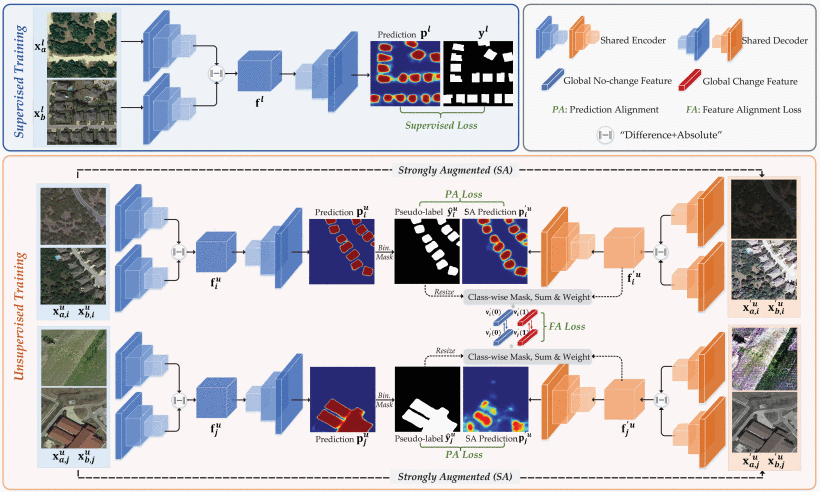
\includegraphics[scale=0.55]{images/FPAframe.png}
  \caption{
    FPA网络框架\cite{Zhang2023FPA}。
  }
  \label{fig:FPAfram}
\end{figure}

(1)类感知特征对齐

类感知特征对齐目的是在训练阶段实现小批量内不同未标记图像对的类内全局特征对齐。具体说来,首先对原始的无标记图像对施加弱增强操作,得到一个弱增强无标记图像对$\left\{\mathbf{x}_{a}^{u}, \mathbf{x}_{b}{ }^{u}\right\}$,并进一步继续对其施加强增强操作得到其对应的强增强图像对$\left\{\mathbf{x'}_{a}^{u}, \mathbf{x'}_{b}{ }^{u}\right\}$:
\begin{equation}
  \label{eq:FPAaug}
  \begin{aligned}
    \mathbf{x}_{a}^{\prime}{ }^{u} & =\operatorname{RandAugment}\left(\mathbf{x}_{a}{ }^{u}\right) \\
    \mathbf{x}_{b}^{\prime}{ }^{u} & =\operatorname{RandAugment}\left(\mathbf{x}_{b}{ }^{u}\right)
  \end{aligned}
\end{equation}

其中$RandAugment(\cdot)$表示从预定义的增强列表中随机抽样两个连接的强增强操作,增强列表如图\ref{fig:FPAstrongAug}所示,包括Identity,Contrast,Autocontrast,Brightness,,Color,,Equalize,Sharpness,Posterize和Solarize等9种常用增强方式,其中a-g分别是(a)原始图像;(b)Identity;(c)Contrast;(d)Autocontrast;(e)Brightness;(f)Color;(g)Equalize;(h)Sharpness;(i)Posterize;(j)Solarize。
\begin{figure}[htb]
  \centering
  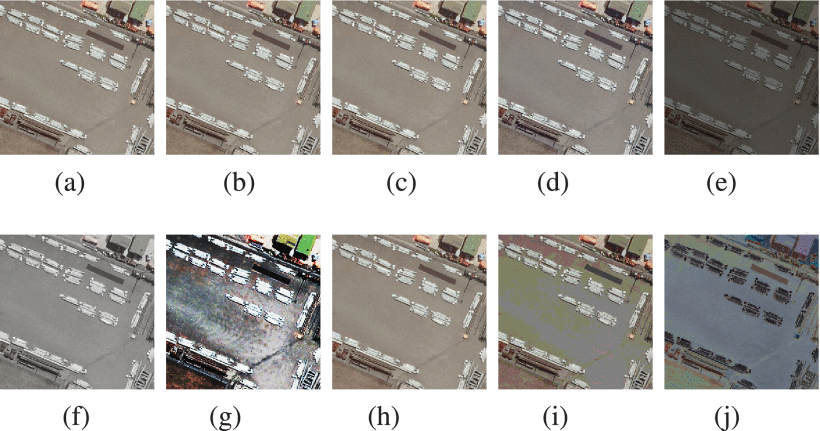
\includegraphics[scale=0.55]{images/Strong_aug.png}
  \caption{
    FPA使用的强增强操作列表\cite{Zhang2023FPA}。
  }
  \label{fig:FPAstrongAug}
\end{figure}

然后,通过编码器分别从$\left\{\mathbf{x}_{a}^{u}, \mathbf{x}_{b}^{u}\right\}$和$\left\{\mathbf{x'}_{a}^{u}, \mathbf{x'}_{b}{ }^{u}\right\}$中提取特征映射$f^u$和强增强特征映射$f'^u$。为了模型训练的鲁棒性,以解码器从$f^u$中提取的弱增强预测映射$p^u$作为伪标签参考,指导在强增强特征图$f'^u$上进行特征对齐操作。为了实现这一步,通过固定阈值筛选掉$p^u$中部分含噪较高的像素预测值:
\begin{equation}
  \label{eq:FPAthresh}
  \mathbf{m}^{u f}(i, j, k)=\left\{\begin{array}{ll}
    1, & \text { if } \quad \mathbf{p}^{u}(i, j, k)>\tau \\
    0, & \text { else }
    \end{array}\right.
\end{equation}

接下来对$m^{u f}$进行最近邻下采样为$\mathbf{m}^{u f} \in \mathbb{R}^{H / s \times W / s \times 2}$以适应强增强特征图$f'^u$的空间分辨率。如此一来便可以基于预测掩码$m^{u f}$和强增强特征映射$f'^u$,提取出分类全局特征向量,记为$\mathbf{v}^{\prime} \in \mathbb{R}^{2 \times C}$,以上过程用公司可表示为如下:
\begin{equation}
  \label{eq:FPAmetafeat}
  \mathbf{v}^{\prime}(k)=\frac{1}{\boldsymbol{w}(k)} * \sum_{i=1}^{H / s} \sum_{j=1}^{W / s} \mathbf{f}^{u}(i, j) * \mathbf{m}^{u f}(i, j, k)
\end{equation}

其中$*$表示逐像素点积运算,$\boldsymbol{w}(k)$为类权像素和,即变化类别的像素总数,计算过程如\ref{eq:FPAsum},$\epsilon = 1e-8$是一个很小的余量,以避免每个类的权重可能为零。
\begin{equation}
  \label{eq:FPAsum}
\boldsymbol{w}(k)=\sum_{i=1}^{H / s} \sum_{j=1}^{W / s} \mathbf{m}^{u f}(i, j, k)+\epsilon
\end{equation}

最后为了实现跨区域的类内特征对齐,FPA通过增加它们的余弦相似度约束来使一个小批中的所有分类全局特征向量彼此对齐,无监督特征对齐损失计算如下:
\begin{equation}
  \label{eq:FPALossf}
  \begin{aligned}
    \mathcal{L}_{u}^{F A}= & \frac{1}{2 B B} \sum_{k=1}^{2} \sum_{i=1}^{B} \sum_{j=1}^{B} \mathbb{I}\left(\boldsymbol{w}_{i}(k)>0, \boldsymbol{w}_{j}(k)>0\right) \\
    & \cdot \frac{1}{2}\left(1-\frac{\mathbf{v}_{i}^{\prime}(k) * \mathbf{v}_{j}^{\prime}(k)}{\left\|\mathbf{v}_{i}^{\prime}(k)\right\|\left\|\mathbf{v}_{j}^{\prime}(k)\right\|+\epsilon}\right)
    \end{aligned}
\end{equation}

其中,$\mathbf{v}_{i}^{\prime}(k)$和$\mathbf{v}_{j}^{\prime}(k)$分别表示当前小批量(B为小批量大小)中第i和第j个未标记图像对的第k类全局特征向量。$\left(\mathbf{v}_{i}^{\prime}(k) * \mathbf{v}_{j}^{\prime}(k) /\left\|\mathbf{v}_{i}^{\prime}(k)\right\|\left\|\mathbf{v}_{j}^{\prime}(k)\right\|\right))$表示$\mathbf{v}_{i}^{\prime}(k)$与$\mathbf{v}_{j}^{\prime}(k)$之间第k类全局特征的余弦相似度,其本身取值范围为[−1,1],为了便于训练FPA将其重映射到了[0,1]。

(2)像素级预测对齐

像素级预测对齐的目的是使强增强图像对的输出与弱增强图像对的输出保持一致,从而使模型获得鲁棒的特征提取能力。为此,FPA中引入了\cite{sohn2020fixmatch}的置信度一致性学习策略,从半监督图像分类任务适用到SSCD的像素级任务。对于从弱增强图像对获取到的像素级的变化概率图$\mathbf{p}^{u}$,按以下方式生成伪标签映射$\hat{\mathbf{y}}^{u} \in \mathbb{R}^{H \times W}$:
\begin{equation}
  \label{eq:FPApesudo}
  \hat{\mathbf{y}}^{u}(i, j)=\underset{k=\{0,1\}}{\arg \max } \mathbf{p}^{u}(i, j, k)
\end{equation}

同样,为了减少噪声伪标签的干扰,对从$\mathbf{p}^{u}$生成的基于置信度的变化掩码$\mathbf{m}^{u p}\in \mathbb{R}^{H \times W}$基于一个固定阈值仅筛选出那些最为可信的预测像素。
\begin{equation}
  \label{eq:FPAfilter}
  \mathbf{m}^{u p}(i, j)=\left\{\begin{array}{ll}
    1, & \text { if } \quad \mathbf{p}^{u}\left(i, j, \hat{\mathbf{y}}^{u}(i, j)\right)>\tau \\
    0, & \text { else. }
    \end{array}\right.
\end{equation}

其中$\tau$是固定阈值的取值,在FPA中默认设置为0.95。

因此,第k个图像对的像素级预测对齐损失,可以表示为公式\ref{eq:FPALossp}和公式\ref{eq:FPALosspavg}:
\begin{equation}
  \label{eq:FPALossp}
  \mathcal{L}_{u}^{P A}(k)=\frac{1}{H W} \sum_{i=1}^{H} \sum_{j=1}^{W} \operatorname{CE}\left(\mathbf{p}^{\prime u}(i, j), \hat{\mathbf{y}}^{u}(i, j)\right) * \mathbf{m}^{u p}(i, j)
\end{equation}
\begin{equation}
  \label{eq:FPALosspavg}
  \mathcal{L}_{u}^{P A}=\frac{1}{B} \sum_{k=1}^{B} \mathcal{L}_{u}^{P A}(k) .
\end{equation}

最终整个无监督训练的损失函数即为类感知特征对齐损失和像素级预测对齐损失的求和:
\begin{equation}
  \label{eq:FPALossu}
  \mathcal{L}_{u}=\mathcal{L}_{u}^{F A}+\mathcal{L}_{u}^{P A} .
\end{equation}
\section{实验指标}
为了更好地衡量所有模型的性能,我们引入了2个广泛使用的变化检测评价指标,包括交并比(Intersection over Union,IoU)和总体精确度(Overall Accuracy,OA)。IoU、OA的取值范围均为0$\%$~100$\%$。对于所有这些指标,该值越大,变化检测性能就越好,但是在变化检测任务中,由于二分类和不平衡的类别不平衡,OA总体上都是一个很高的值。它们的计算表述如下:
\begin{equation}
  \label{eq:IoU}
  I o U=\frac{T P}{T P+F P+F N}
\end{equation}
\begin{equation}
  \label{eq:OA}
  O A=\frac{T P+T N}{T P+T N+F N+F P}
\end{equation}

其中$TP$和$TN$分别表示正确识别的变化像素数和未变化像素数。相反,$FP$表示未发生变化的像素被错误地分类为变化的像素的数量,$FN$表示发生变化的像素被错误地识别为未变化的像素的数量。此外,由于我们更关注变化区域的预测性能,并且变化类和背景类极度不平衡,因此在实验中使用变化类的$IoU$ ($IoU_c$)作为评价指标。
\section{实验数据集介绍}
本文中所有方法都在十个基准公开变化检测数据集上进行了实验,分别是LEVIR-CD\cite{chen2020levircd}、LEVIR-CD+\cite{chen2020levircd}、WHU-CD\cite{ji2018whu}、EGY-CD\cite{holail2023EGYCD}、HRCUS-CD\cite{zhang2023HRCUS}、Change Detection Dataset(CDD)\cite{Lebedev2018CDD}、GZ-CD\cite{peng2021SemiCDNet}、DSIFN-CD\cite{zhang2020dsifn}、SYSU-CD\cite{shi2022SYSU}和CL-CD\cite{liu2022CLCD}。其中,这些数据集涵盖了不同的分辨率(0.03m-2.0m)、不同的数据大小(2400至20000对)、不同的标注类别(二值建筑物或多类)、不同的图像对时间跨度(1年-16年),汇总如表\ref{datasets}所示,二值建筑物变化检测数据集部分样例展示如图\ref{fig:building_sample}所示,多类变化检测数据集部分样例展示如图\ref{fig:mutil_sample}所示。
\begin{table*}[!htbp]
  \centering
  \caption{本文所使用的公开数据集。}
  \begin{tabular}{c|c|c|c|c|c|c}
  \toprule[1pt]
  % \rowcolor[HTML]{DAE8FC}
  \rowcolor[HTML]{ECF4FF}
  \textbf{变化类别} &
    \textbf{数据集} &
    \textbf{空间分辨率} &
    \textbf{大小} &
    \textbf{样本数量} &
    \textbf{时间跨度} &
    \textbf{链接}
    \\
    % \hline
    \midrule
   & LEVIR-CD  \cite{chen2020levircd}  & 0.5m & 1024 $\times$ 1024   & 637 & 5到14年 &\href{https://justchenhao.github.io/LEVIR/}{\textcolor{blue}{Link}} \\
   \cline{2-7}
   & LEVIR-CD+ \cite{chen2020levircd}  & 0.5m & 1024 $\times$ 1024   & 985  & 5到14年
  &\href{https://justchenhao.github.io/LEVIR/}{\textcolor{blue}{Link}}\\
   \cline{2-7}
    &WHU-CD \cite{ji2018whu}&
    0.2m &
    15354$\times$32507 &
    1 &
    2012年至2016年
  &\href{http://study.rsgis.whu.edu.cn/pages/download/building_dataset.html}{\textcolor{blue}{Link}}\\
  \cline{2-7}
   & GZ-CD \cite{peng2021SemiCDNet}&
    0.55m &
    Varying &
    19 &
    2006年至2019年
  &\href{https://github.com/daifeng2016/Change-Detection-Dataset-for-High-Resolution-Satellite-Imagery}{\textcolor{blue}{Link}}\\
  \cline{2-7}
     & EGY-BCD \cite{holail2023EGYCD}&
    0.25m &
    256 $\times$ 256 &
    6091 &
    2015年至2022年
  &\href{https://github.com/oshholail/EGY-BCD}{\textcolor{blue}{Link}}\\
  \cline{2-7}
  \multirow{-5}{*}{\textbf{\begin{tabular}[c]{@{}c@{}} 建筑物\end{tabular}}} &
  HRCUS-CD \cite{zhang2023HRCUS}&
    0.5m &
    256 $\times$ 256 &
    11388 &
    混合
  &\href{https://github.com/zjd1836/AERNet}{\textcolor{blue}{Link}}\\
    \midrule
    % \hline
   & CDD\cite{Lebedev2018CDD}   & 0.03m-1.0m & 256$\times$256  & 16000    & 混合
   &\href{https://drive.google.com/uc?id=0B-IG2NONFdciOWY5QkQ3OUgwejQ&export=download}{\textcolor{blue}{Link}} \\
   \cline{2-7}
   & DSIFN-CD \cite{zhang2020dsifn} &Unknown & 512$\times$512   & 3940    & 未知
  &\href{https://github.com/GeoZcx/A-deeply-supervised-image-fusion-network-for-change-detection-in-remote-sensing-images/tree/master/dataset}{\textcolor{blue}{Link}} \\
   \cline{2-7}
   & SYSU-CD\cite{shi2022SYSU} &0.5m & 256$\times$256 & 20000  & 2007年至2014年
   &\href{https://github.com/liumency/SYSU-CD}{\textcolor{blue}{Link}} \\
   \cline{2-7}
  \multirow{-4}{*}{\textbf{\begin{tabular}[c]{@{}c@{}} 多类\end{tabular}}}
   & CL-CD \cite{liu2022CLCD} &0.5-2.0m & 512$\times$512 & 600  & 2017年至2019年
   &\href{https://github.com/liumency/CropLand-CD}{\textcolor{blue}{Link}} \\
  \midrule
  \end{tabular}
  \label{datasets}
  \end{table*}

\textbf{LEVIR-CD数据集}:该数据集是一个综合性的遥感建筑变化检测数据集,由637对超高分辨率的谷歌地球图像块组成,每个块的空间分辨率为0.5m,尺寸为$1024\times1024$像素。这些双时相图像来自美国德克萨斯州七个城市的20个不同地点,双时相图像拍摄于2002年至2018年间,时间跨度在5到14年。经过切割之后,该数据集的分布是这样的:训练集占比为70$\%$(7120对),验证集占比为10$\%$(1024对),测试集占另外20$\%$(2048对)。

\textbf{LEVIR-CD+数据集}:LEVIR-CD+是对现有LEVIR-CD数据集的一个扩展版本,包含的样本数量扩充到985对$1024\times1024$像素的图像对,其中来自LEVIR-CD的637对用于训练,我们将其中的10$\%$用于验证,其余扩展的385对用于测试。

\textbf{WHU-CD数据集}:原始数据集由单个双时相图像对组成,其中包括2012年和2016年拍摄的新西兰克赖斯特彻奇的两张航拍图像。以同样的切割方式,我们将其分成7434个不重叠的图像对,每个图像对的大小为$256\times256$像素。训练、验证和测试数据集分别由5947、743和744对图像组成。

\textbf{GZ-CD数据集}:GZ-CD数据集的双时相图像收集于2006年至2019年,覆盖中国广州郊区。共收集了19幅不同尺寸的红、绿、蓝波段空间分辨率为0.55m的超分辨率图像,注释集中在建筑物变化上。经过切割成统一尺寸之后,共包含3603对样本,其中训练样本2882对,验证样本360对,测试样本361对。

\textbf{EGY-BCD数据集}:EGY-CD数据集包含6091张2015 - 2022年拍摄的$256 \times 256$像素的图像对,空间分辨率为0.25m/像素,主要标注了埃及4个城市和沿海地区的建筑变化区域。不用额外处理,我们将其中70$\%$用于训练,20$\%$用于验证,剩下的10$\%$用于测试。

\textbf{HRCUS-CD数据集}:该数据集由11388对高分辨率遥感图像组成,裁剪为$256 \times 256$像素,空间分辨率为0.5m。主要分为两个征集区,一个是城市建成区,时间跨度从2019年到2022年,建筑变化面积较少;另一个是正在建设的新城区,从2010年到2018年,包含农田、山地等多种地貌,建筑物变化面积较大。

\textbf{CDD数据集}:CDD数据集包含16000对$256\times256$像素的双时相图像对,像素分辨率从0.03到1米不等。所有这些双时间图像都是从谷歌地球收集的7对$4725\times2700$像素的季节性变化图像对中裁剪出来的。分别有10000对、3000对和3,000对用于训练、验证和测试。

\textbf{DSIFN-CD数据集}:DSIFN-CD是在谷歌地球上人工采集的,它由覆盖中国6个城市(北京、成都、深圳、重庆、武汉、西安)的6幅大型双时相超高分辨率图像组成。其中五个大图像对(北京、成都、深圳、重庆、武汉)被裁剪成394个子图像对,大小为$512\times512$像素。经过数据增强后,得到3940对双相图像。将西安图像对裁剪为48个子图像对进行测试。最终切割为统一的$256\times256$像素之后,训练数据集中有14400对图像,验证数据集中有1360对图像,测试数据集中有192对图像。

\textbf{SYSU-CD数据集}:该数据集由2007年至2014年在香港拍摄的20000对$256\times256$像素、 空间分辨率为0.5米航拍图像组成。数据集中的主要变化类型包括:(a)新建城市建筑;(b)郊区扩张;(c)施工前基础工作;(d)植被变化;(e)扩大道路;(f)近海建筑。我们将其中70$\%$的样本用于训练,20$\%$的样本用于验证,剩下的10$\%$的样本集用于测试。

\textbf{CL-CD数据集}:CL-CD数据集由600对农田变化样本图像组成,其中320对用于训练,120对用于验证,120对用于测试。CL-CD的双时相影像是2017年和2019年由中国广东省高分二号卫星采集的,空间分辨率范围为0.5-2 m。每组样本由两个$512 \times 512$像素图像和对应的字段变化的二进制标签组成。CL-CD中指出的主要变化类型包括建筑物、道路、湖泊和裸露的土地。我们将训练、验证、测试集都切割为$256\times256$大小之后进行使用。
\begin{figure}[htb]
  \centering
  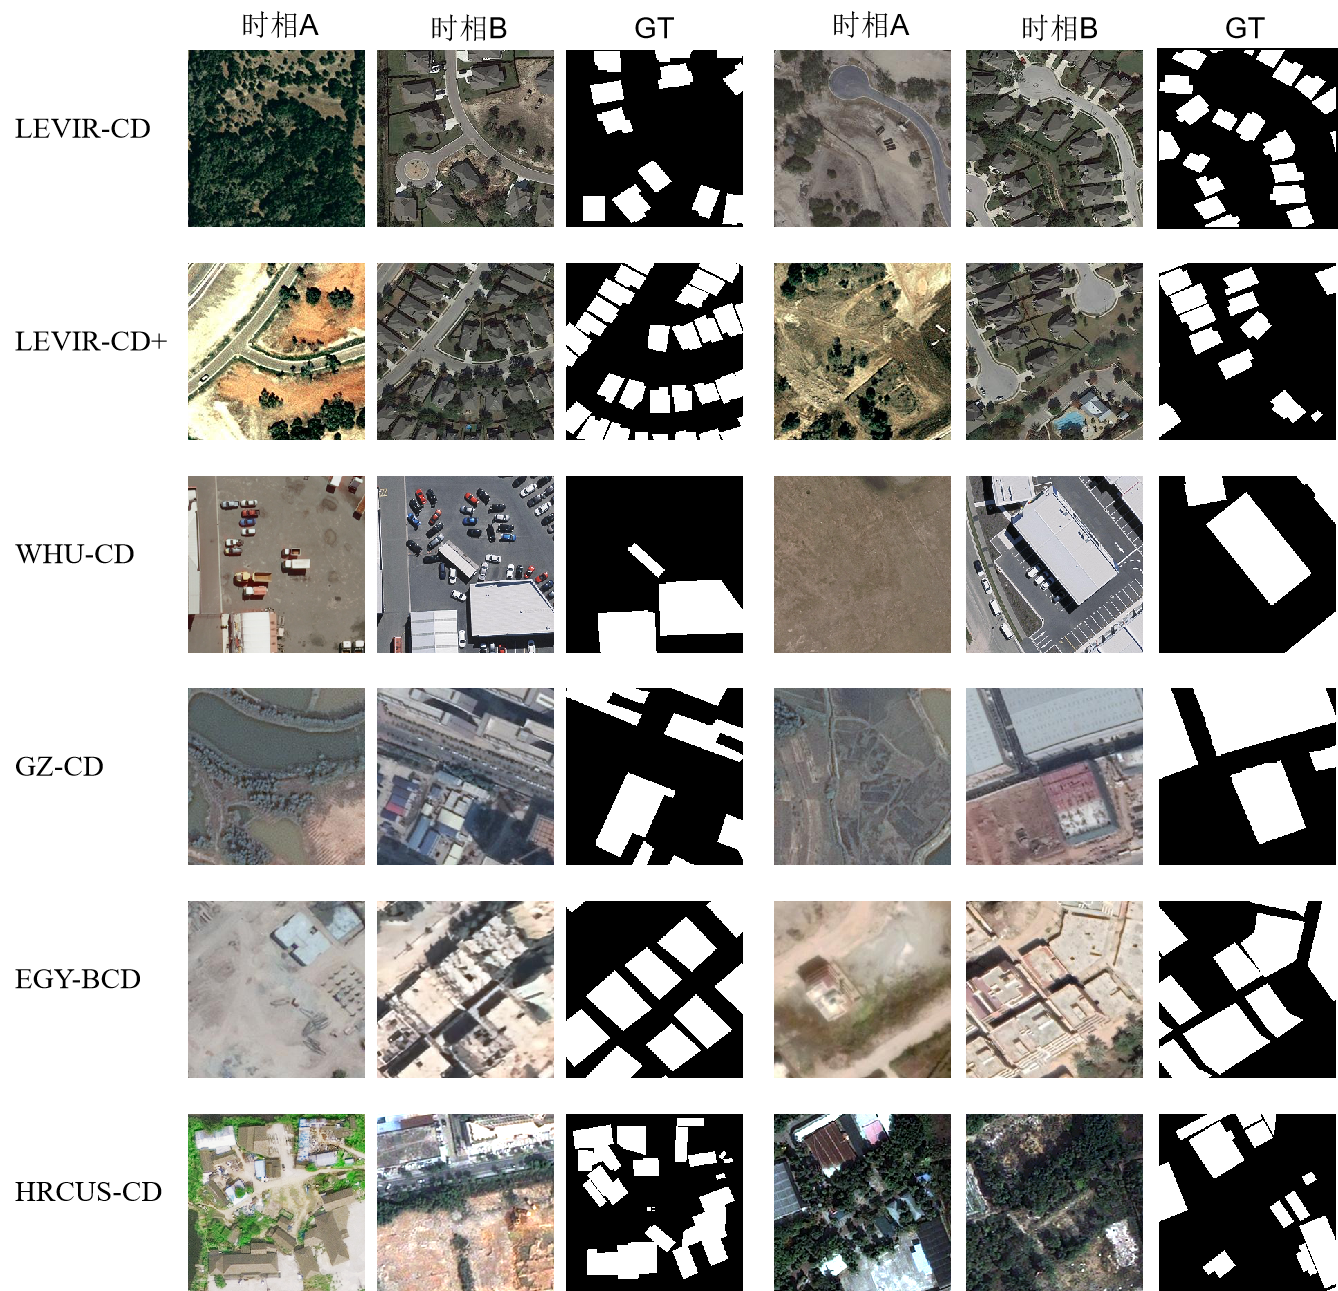
\includegraphics[scale=0.65]{images/building_sample.png}
  \caption{
    建筑物变化检测数据集部分样例图。
  }
  \label{fig:building_sample}
\end{figure}

\begin{figure}[htb]
  \centering
  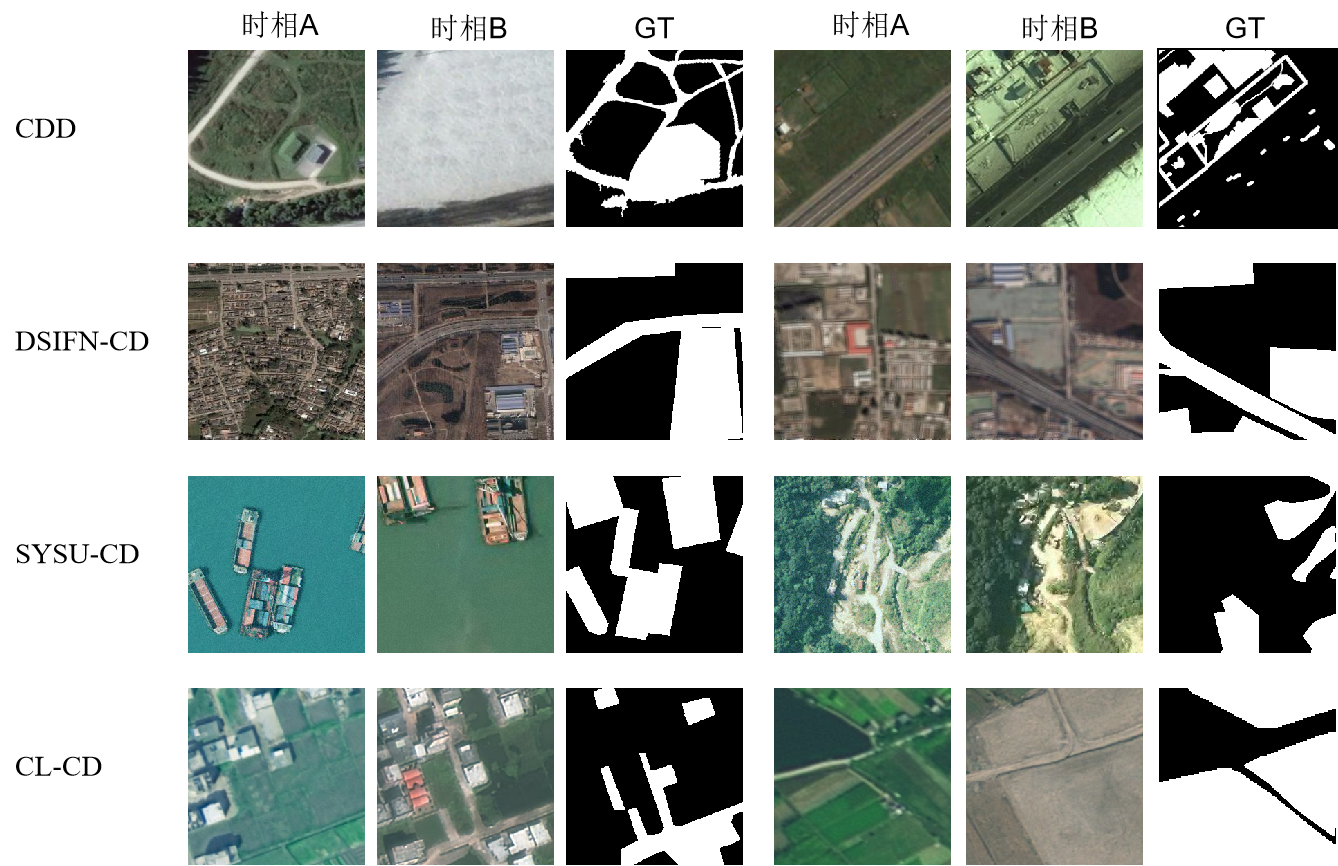
\includegraphics[scale=0.65]{images/mutil_sample.png}
  \caption{
    多类变化检测数据集部分样例图。
  }
  \label{fig:mutil_sample}
\end{figure}

\section{本章小结}
本章主要介绍了本文研究内容的相关技术,首先简要介绍了卷积神经网络,主要包括本文中用到的ResNet模型。随后阐述了Vison Transformer模型的架构和原理。接着介绍了本文研究实验中使用的变化检测的 2 种最常用的评价指标。最后介绍了本文使用的十个公开数据集,所有实验均在这十个数据集上进行训练和验证。
\chapter{基于伪标签评估的自适应半监督变化检测算法}
\section{引言}
\section{基于伪标签评估的自适应半监督变化检测框架}
\subsection{整体框架}
\subsection{伪标签评估指标设计}
\subsection{自适应样本增强机制}
\subsection{自适应师生模型参数更新机制}
\section{实验结果及分析}
\subsection{变化检测数据集介绍}
\subsection{评估指标}
\subsection{实验设置}
\subsection{对比试验}
\subsection{消融实验}
\section{本章小结}


\chapter{基于SAM改善伪标签的半监督变化检测算法}
\section{引言}
\section{基于SAM改善伪标签的半监督变化检测框架}
\subsection{整体框架}
\subsection{基于双时分割掩码差分的伪标签生成}
\subsubsection{像素级差分算法}
\subsubsection{实例级差分算法}
\subsection{基于双时特征差分的伪标签生成}
\section{实验结果及分析}
\subsection{实验设置}
\subsection{对比试验}
\subsection{消融实验}
\section{本章小结}

\chapter{基于APE的单模型半监督变化检测算法}
\section{引言}
\section{基于APE的单模型半监督变化检测框架}
\subsection{整体框架}
\subsection{基于查询的自动伪标签生成}
\section{实验结果及分析}
\subsection{实验设置}
\subsection{对比试验}
\subsection{消融实验}
\section{本章小结}

\chapter{总结与展望}
\section{本文工作总结}
\section{未来研究展望}

\cleardoublepage
%%=============================================================================%
%% 参考文献以及附录
%%-----------------------------------------------------------------------------%
%% \bibliographystyle{nputhesis}                               % GB/T 7714-2015 格式
\bibliographystyle{nputhesis-noslash}                       % 参考文献改进格式
\bibliography{reference}                                    % 参考文献
\appendix

%%=============================================================================%
%% 文档附页部分(致谢、参加科研情况、知识产权与原创性声明)
%%-----------------------------------------------------------------------------%
\backmatter                                                 % 文档附页部分
%%-----------------------------------------------------------------------------%
\begin{acknowledgements}                                    % 致谢开始
感谢我的老师和我的朋友们……
\end{acknowledgements}                                      % 致谢结束
%%-----------------------------------------------------------------------------%
\begin{accomplishments}                                     % 参加科研情况开始
    [1] ...
\end{accomplishments}                                       % 参加科研情况结束
%%-----------------------------------------------------------------------------%
\makestatement                                              % 知识产权与原创性声明
%%=============================================================================%
%% 文档结束
%%-----------------------------------------------------------------------------%
\end{document}
%%=============================================================================%


%%
%% This work consists of the file  yanputhesis.dtx
%% and the derived files           yanputhesis.ins,
%%                                 yanputhesis.pdf,
%%                                 yanputhesis.cls.
%%
%%
%% End of file `yanputhesis-sample.tex'.
